\documentclass[12pt, oneside]{article}
\usepackage[top = 1in, bottom = 1in, left =1in, right = 1in]{geometry}
\usepackage{titling}
\usepackage{graphicx}
\usepackage{subfig}
\usepackage{datatool}

\setlength{\droptitle}{-5em}	% Saves title space, uses package titling

\title{phox Results for Fe$_{0.80}$Ni$_{0.10}$Ni$_{0.10}$ with manual fitting}
\author{Rachel Morrison}
\date	{\today}
\begin{document}
\maketitle
\tableofcontents

\begin{figure}[h!]
\centering
\subfloat{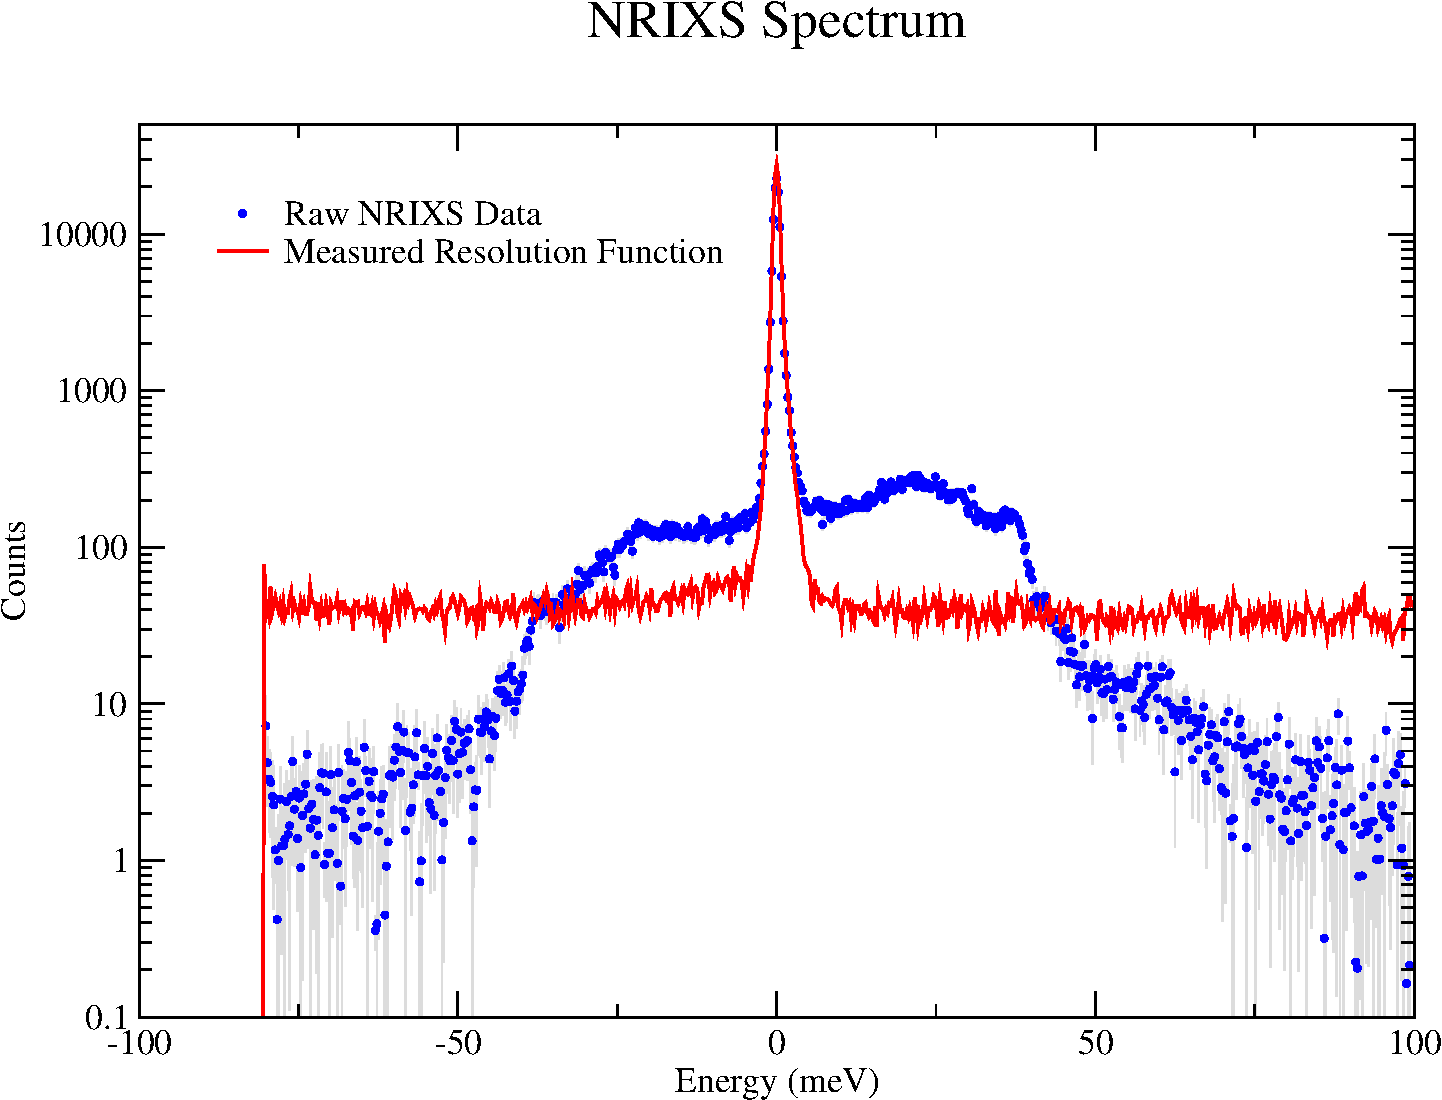
\includegraphics[width=8.0cm]{2013Nov_DAC14_P1//PhoxFigures/NRIXS_FeNiSi_DAC14_P1.pdf}} \quad
\subfloat{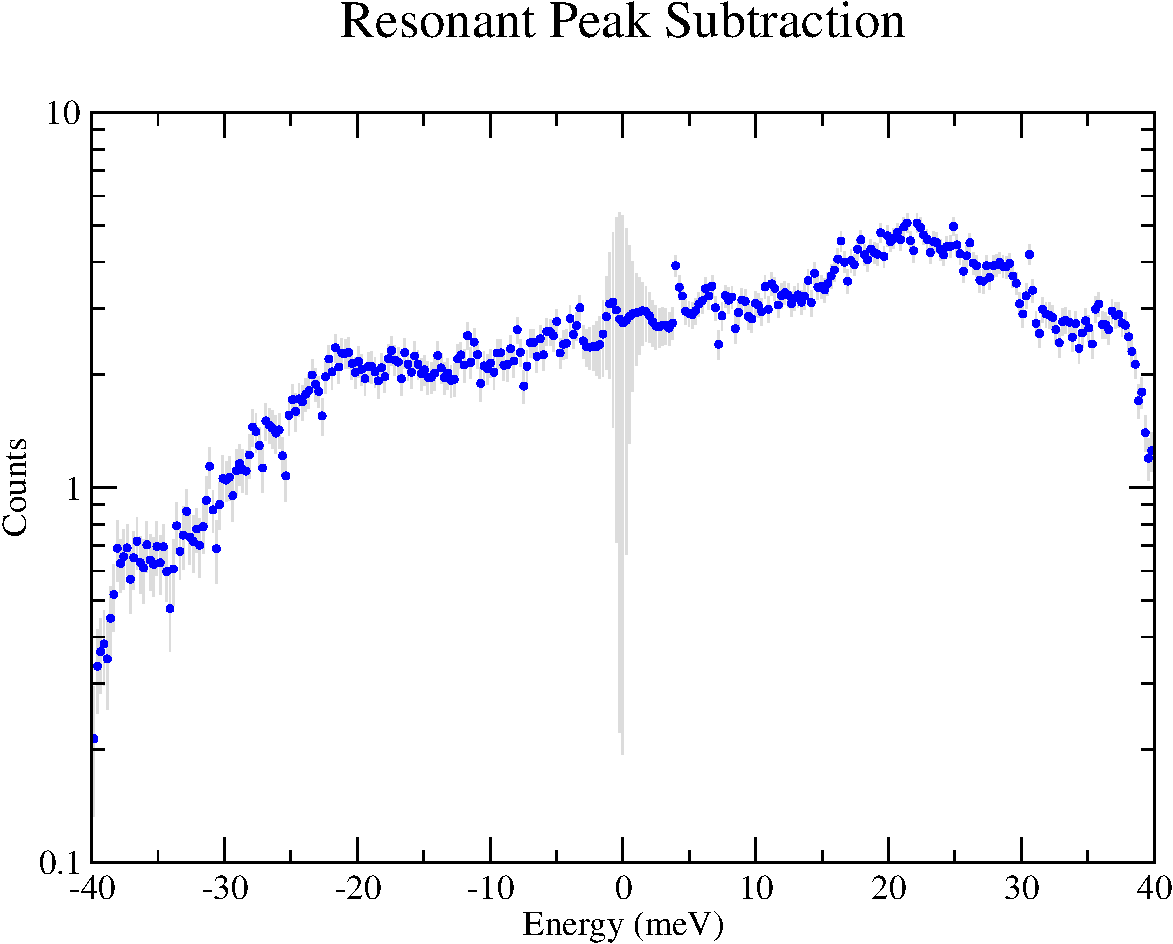
\includegraphics[width=7.5cm]{2013Nov_DAC14_P1//PhoxFigures/PeakSub_FeNiSi_DAC14_P1.pdf}} \\
\subfloat{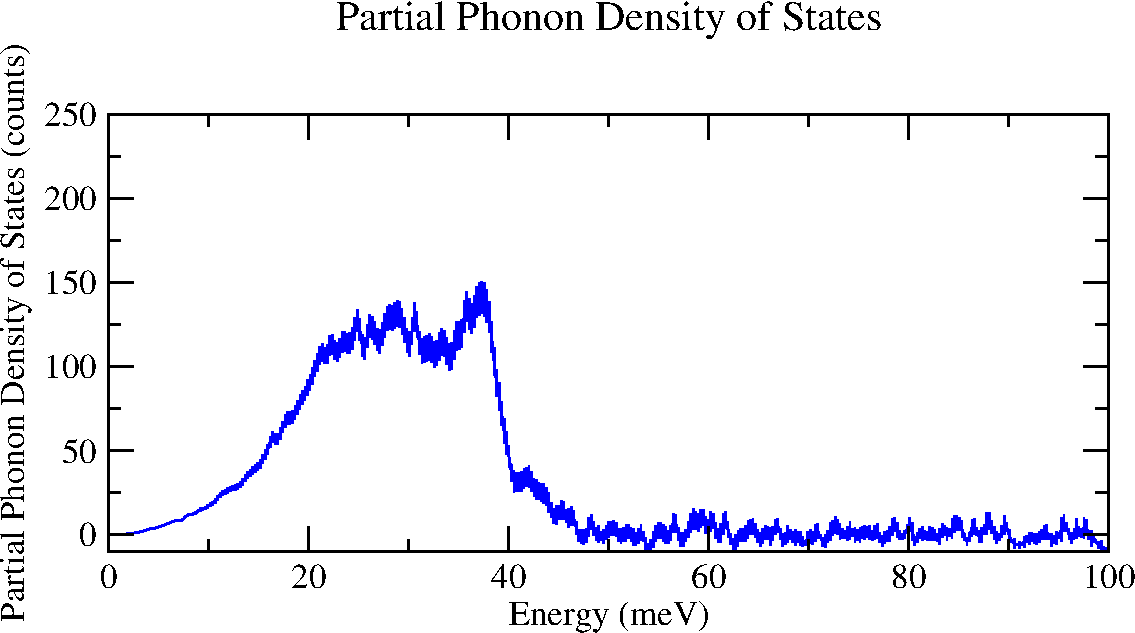
\includegraphics[width=7.5cm]{2013Nov_DAC14_P1//PhoxFigures/PDOS_FeNiSi_DAC14_P1.pdf}} \quad
\subfloat{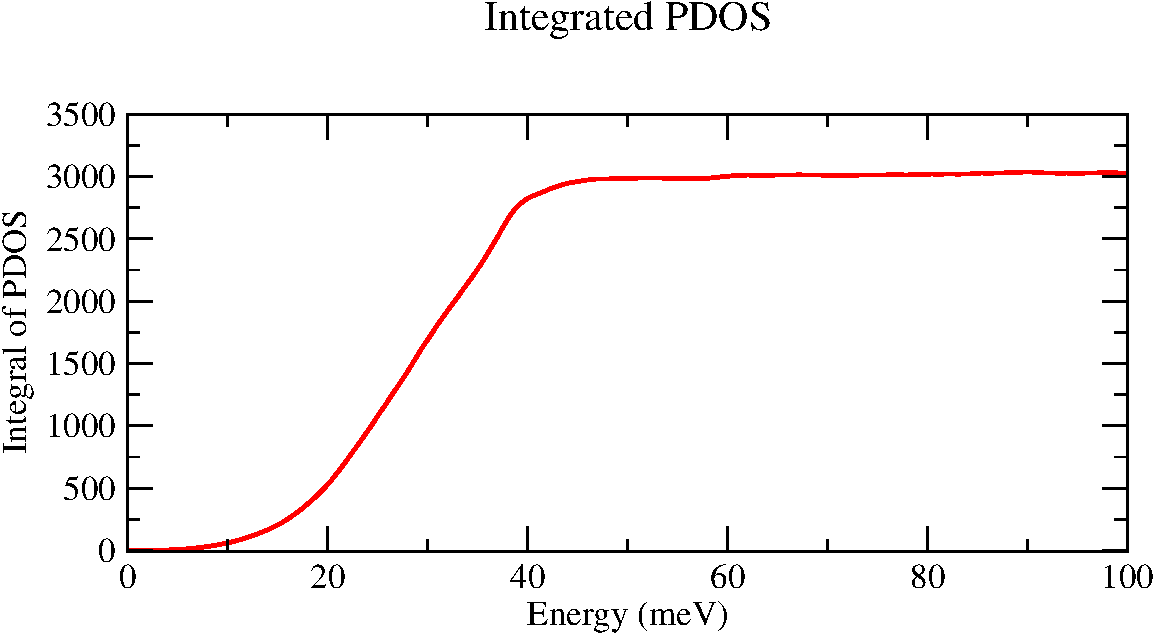
\includegraphics[width=7.5cm]{2013Nov_DAC14_P1//PhoxFigures/IntPDOS_FeNiSi_DAC14_P1.pdf}} \\
\subfloat{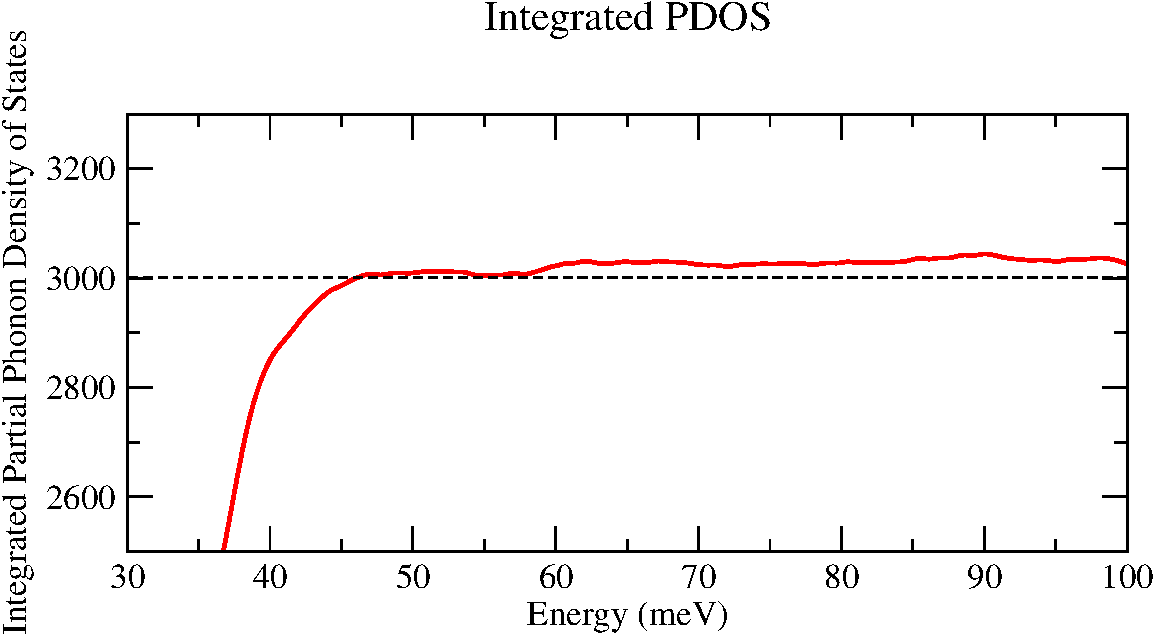
\includegraphics[width=8.0cm]{2013Nov_DAC14_P1//PhoxFigures/IntPDOSZoom_FeNiSi_DAC14_P1.pdf}} \quad
\subfloat{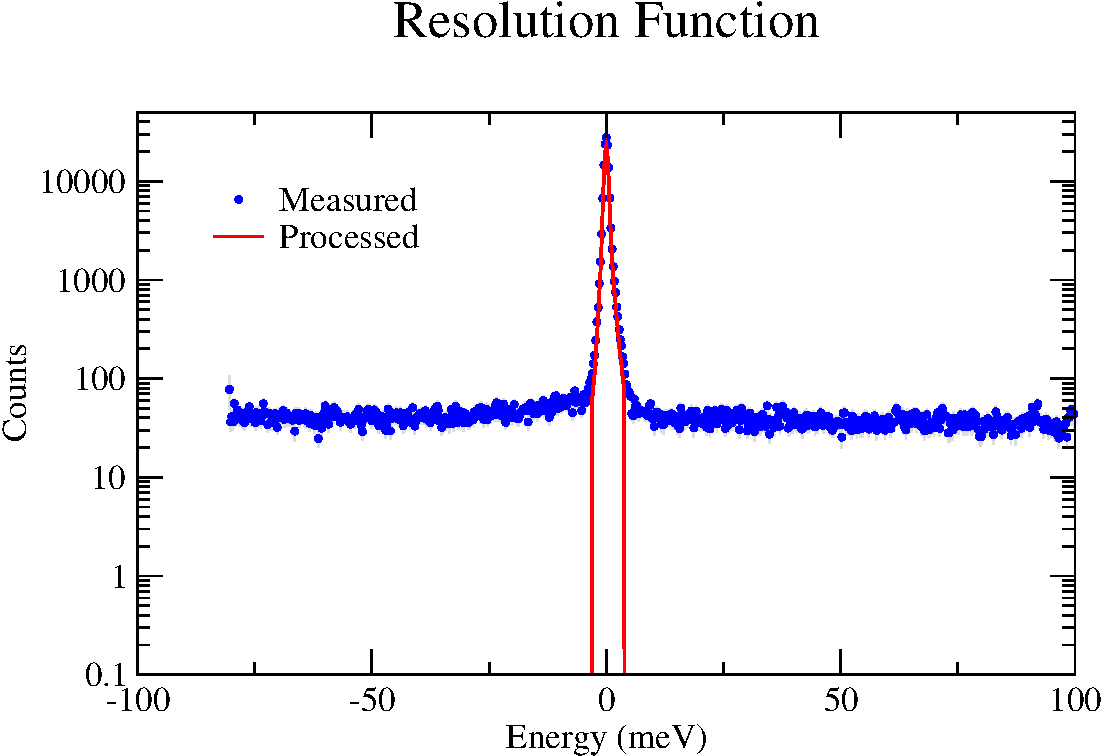
\includegraphics[width=7.5cm]{2013Nov_DAC14_P1//PhoxFigures/ResPeak_FeNiSi_DAC14_P1.pdf}}
\caption{PHOENIX phox data for Fe$_{0.80}$Ni$_{0.10}$Ni$_{0.10}$ data point FeNiSi\_DAC14\_P1.}
\label{fig:cont}
\end{figure}

\begin{figure}[h!]
\centering
\subfloat{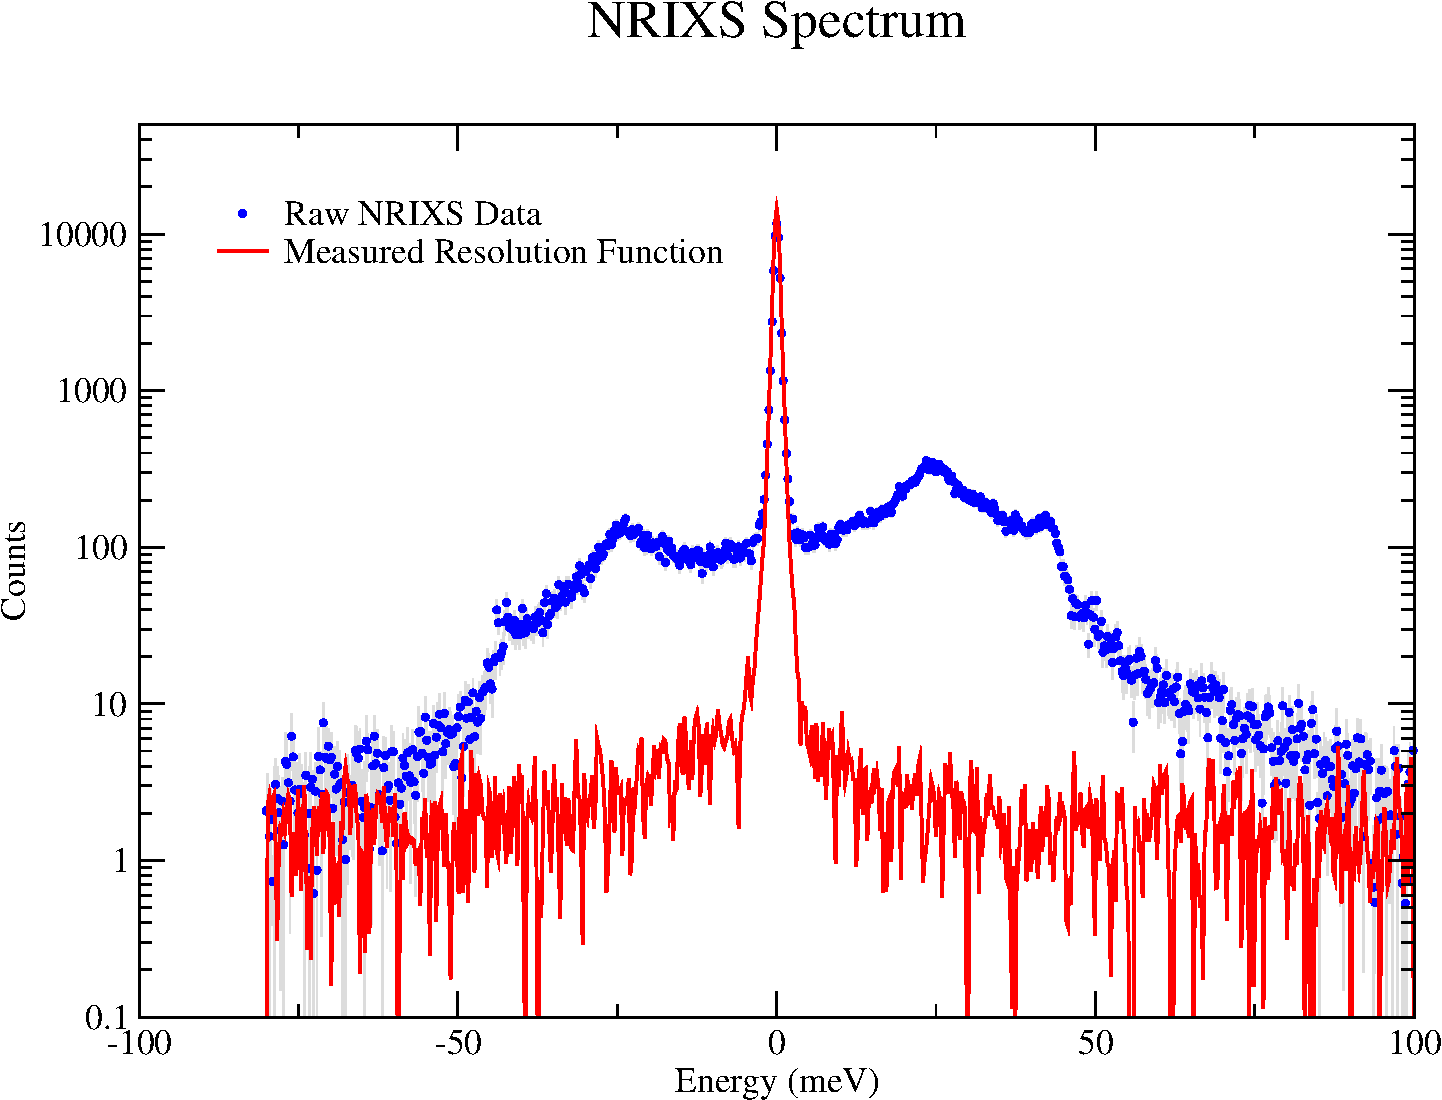
\includegraphics[width=8.0cm]{2014Feb_DAC13_P1//PhoxFigures/NRIXS_FeNiSi_DAC13_P1.pdf}} \quad
\subfloat{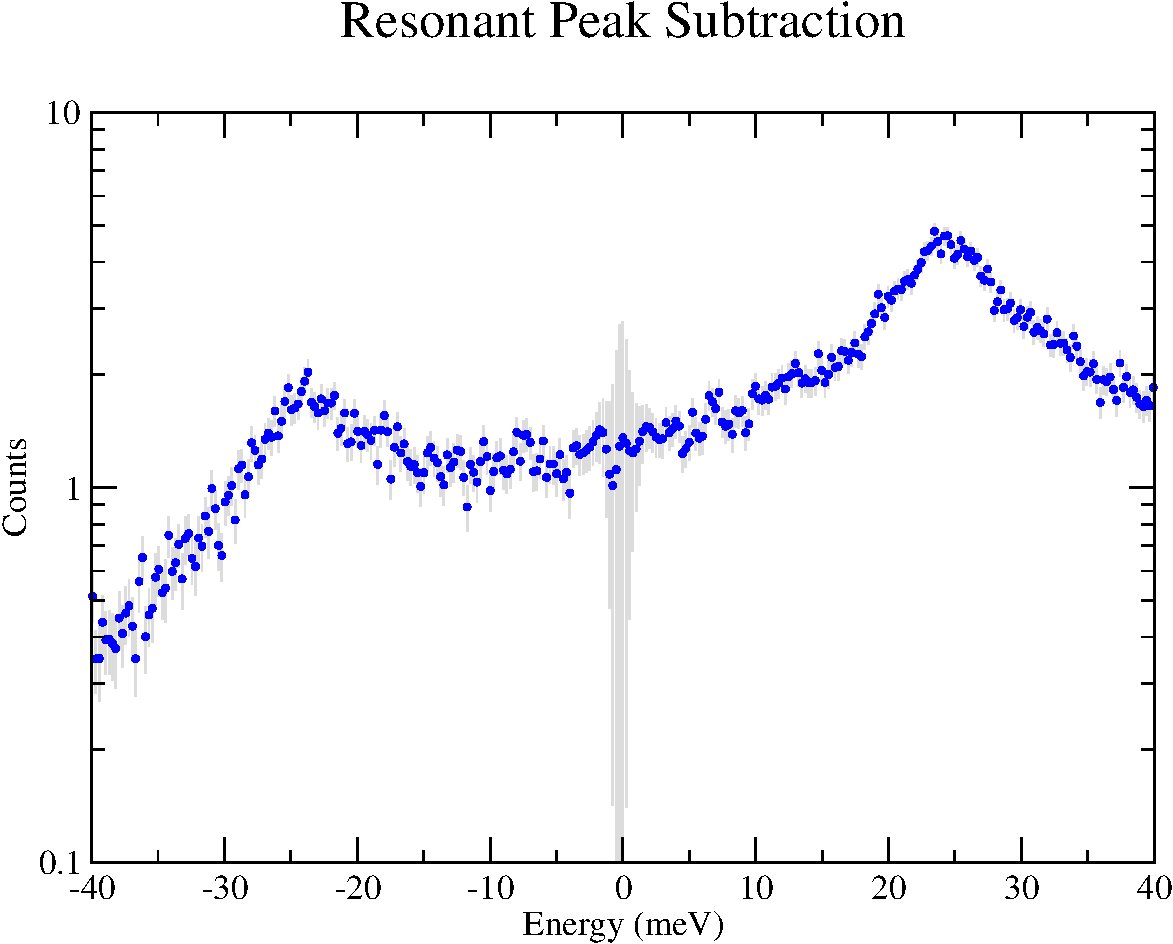
\includegraphics[width=7.5cm]{2014Feb_DAC13_P1//PhoxFigures/PeakSub_FeNiSi_DAC13_P1.pdf}} \\
\subfloat{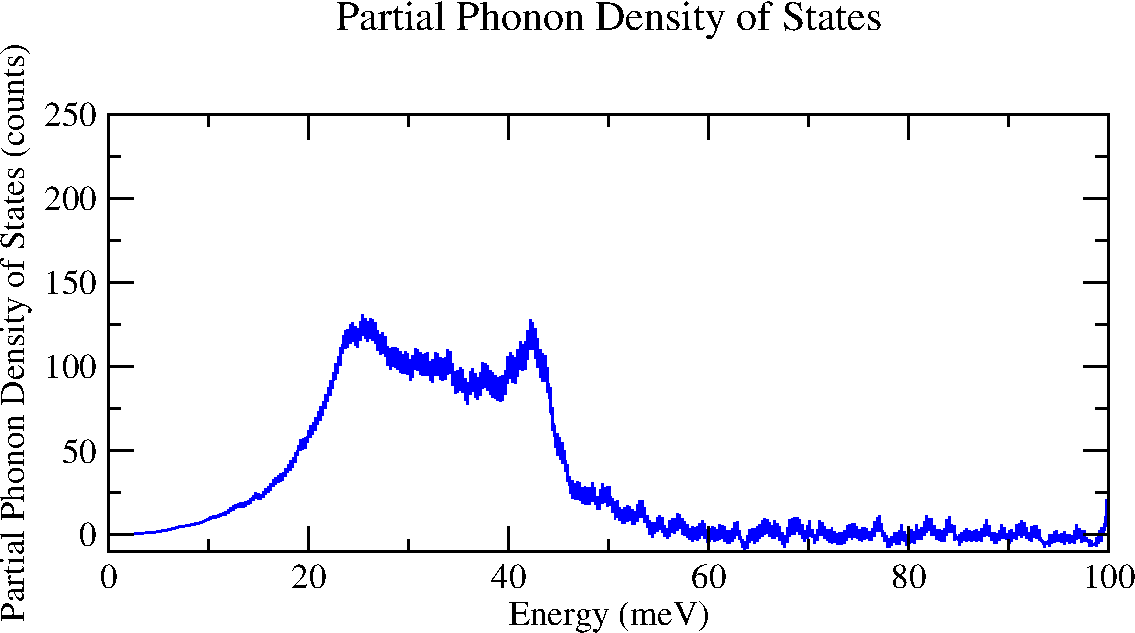
\includegraphics[width=7.5cm]{2014Feb_DAC13_P1//PhoxFigures/PDOS_FeNiSi_DAC13_P1.pdf}} \quad
\subfloat{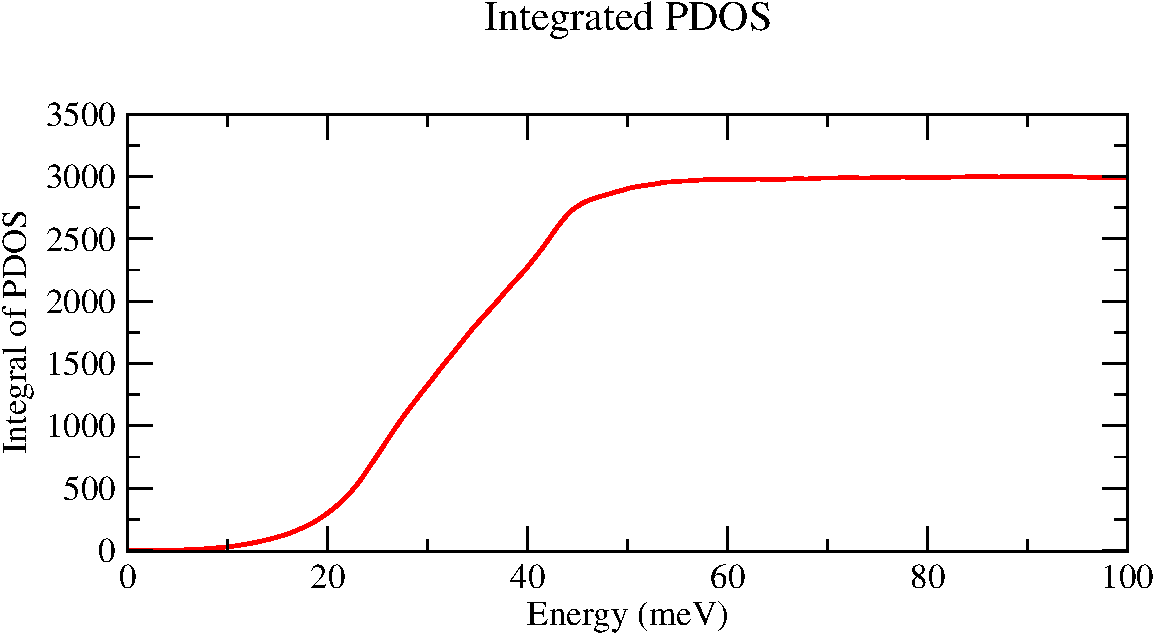
\includegraphics[width=7.5cm]{2014Feb_DAC13_P1//PhoxFigures/IntPDOS_FeNiSi_DAC13_P1.pdf}} \\
\subfloat{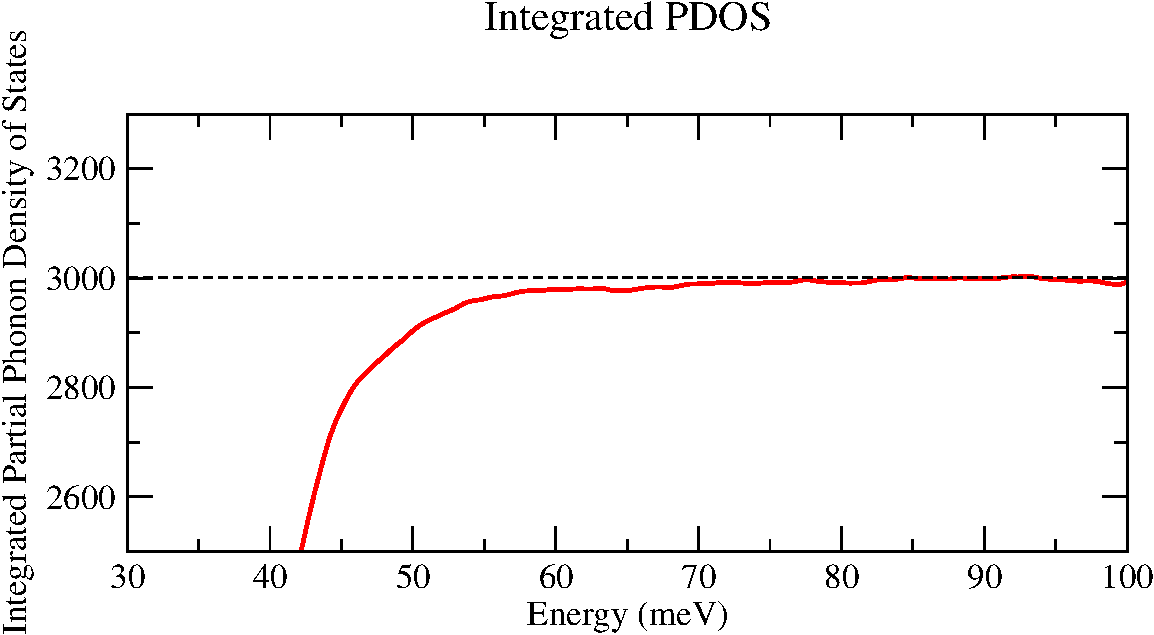
\includegraphics[width=8.0cm]{2014Feb_DAC13_P1//PhoxFigures/IntPDOSZoom_FeNiSi_DAC13_P1.pdf}} \quad
\subfloat{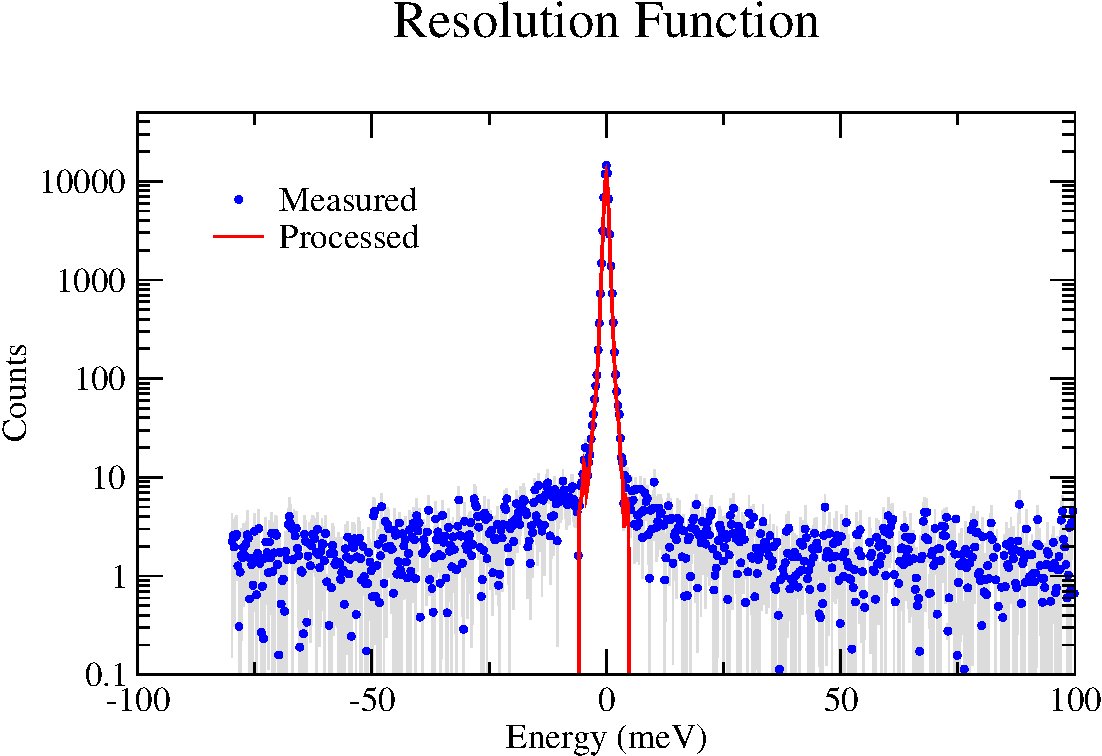
\includegraphics[width=7.5cm]{2014Feb_DAC13_P1//PhoxFigures/ResPeak_FeNiSi_DAC13_P1.pdf}}
\caption{PHOENIX phox data for Fe$_{0.80}$Ni$_{0.10}$Ni$_{0.10}$ data point FeNiSi\_DAC13\_P1.}
\label{fig:cont}
\end{figure}

\begin{figure}[h!]
\centering
\subfloat{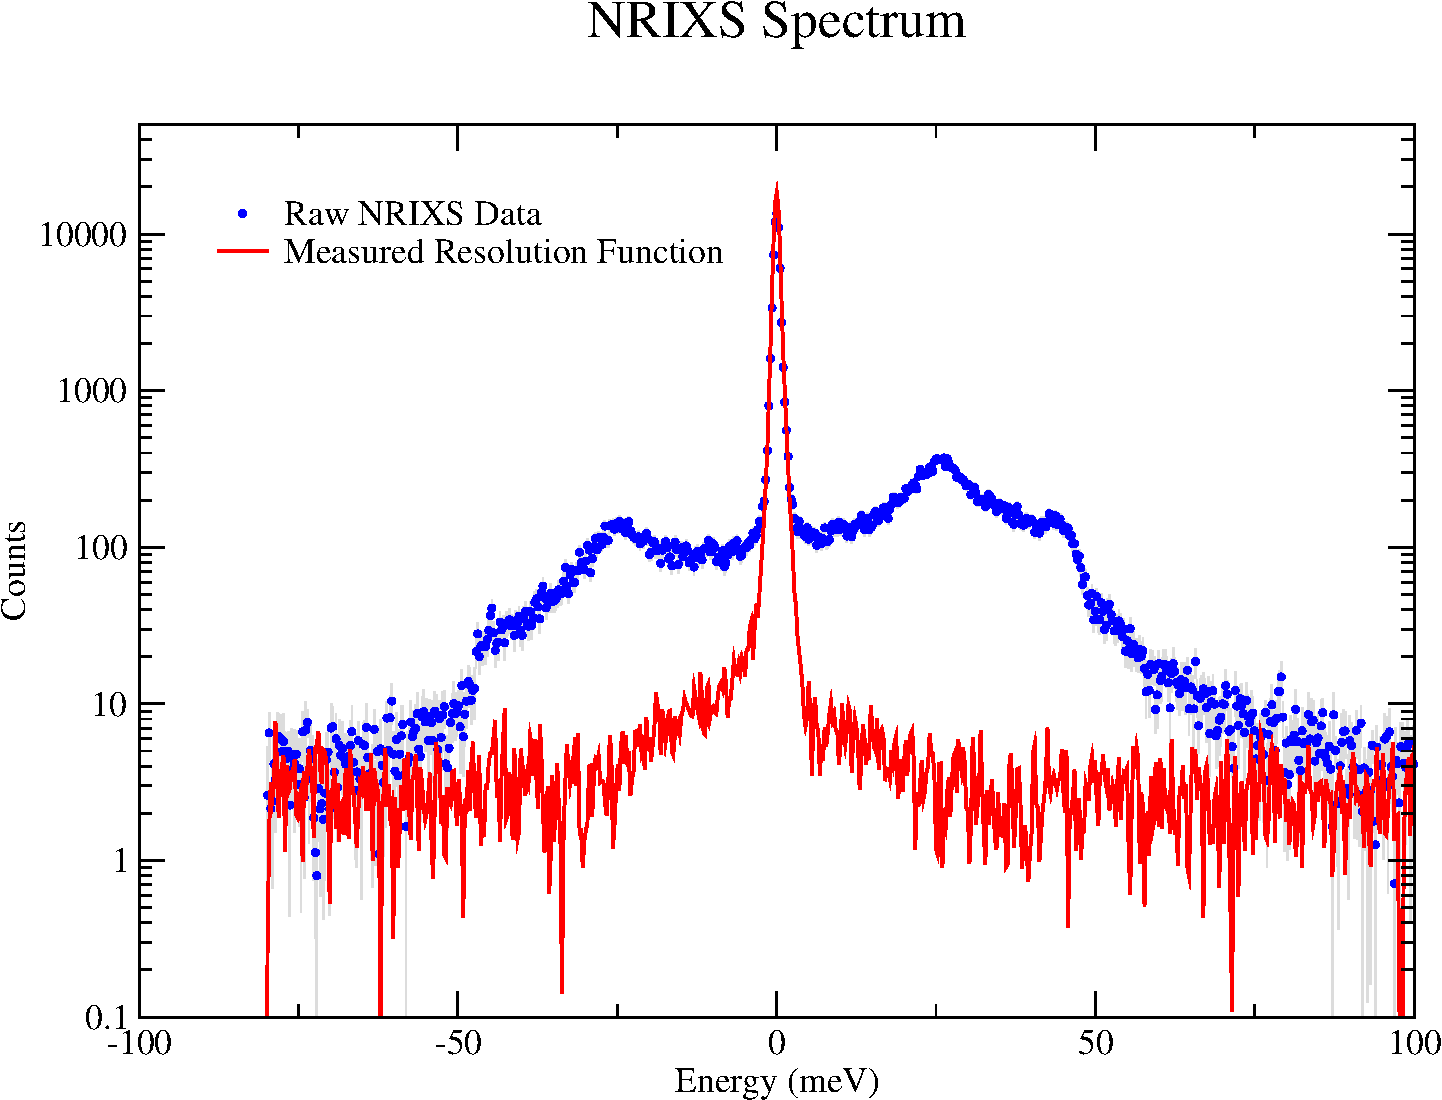
\includegraphics[width=8.0cm]{2014Feb_DAC13_P2//PhoxFigures/NRIXS_FeNiSi_DAC13_P2.pdf}} \quad
\subfloat{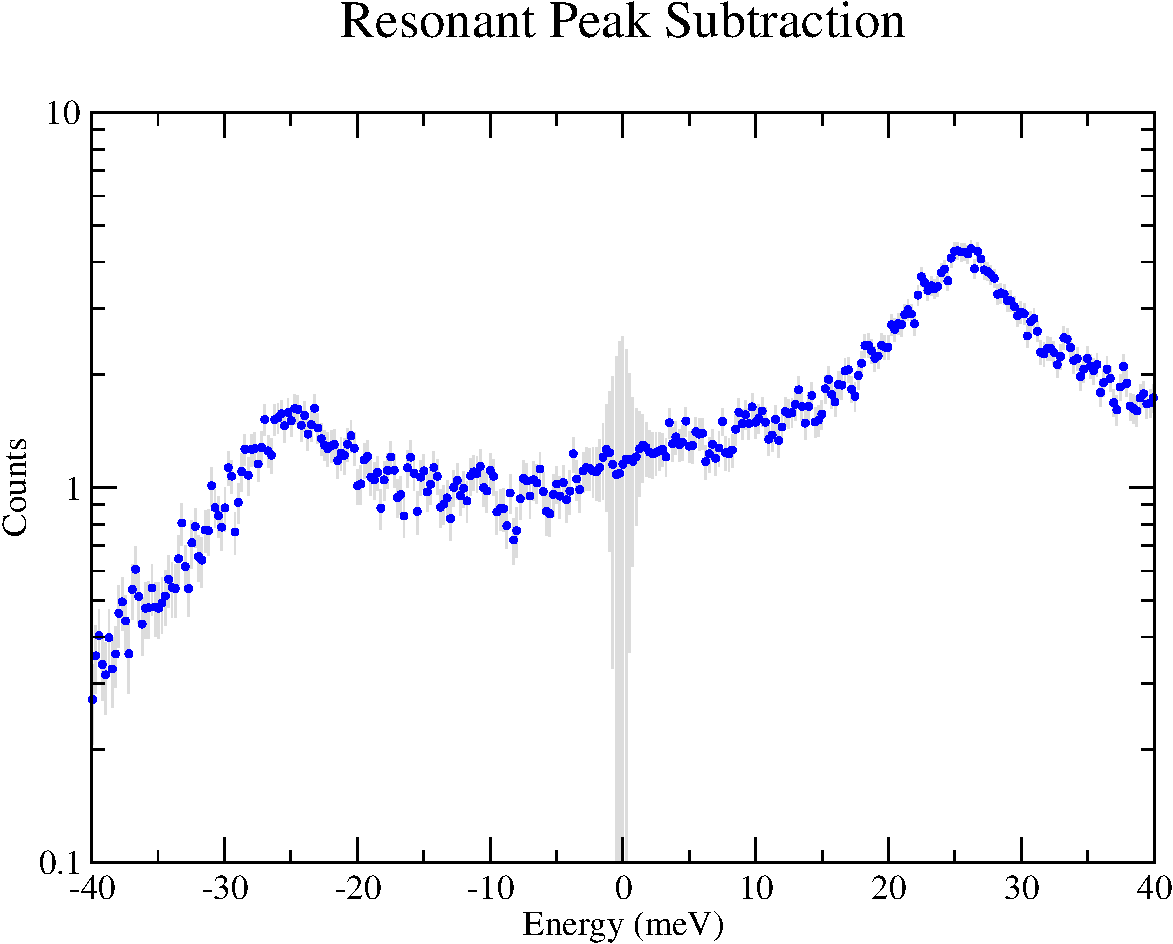
\includegraphics[width=7.5cm]{2014Feb_DAC13_P2//PhoxFigures/PeakSub_FeNiSi_DAC13_P2.pdf}} \\
\subfloat{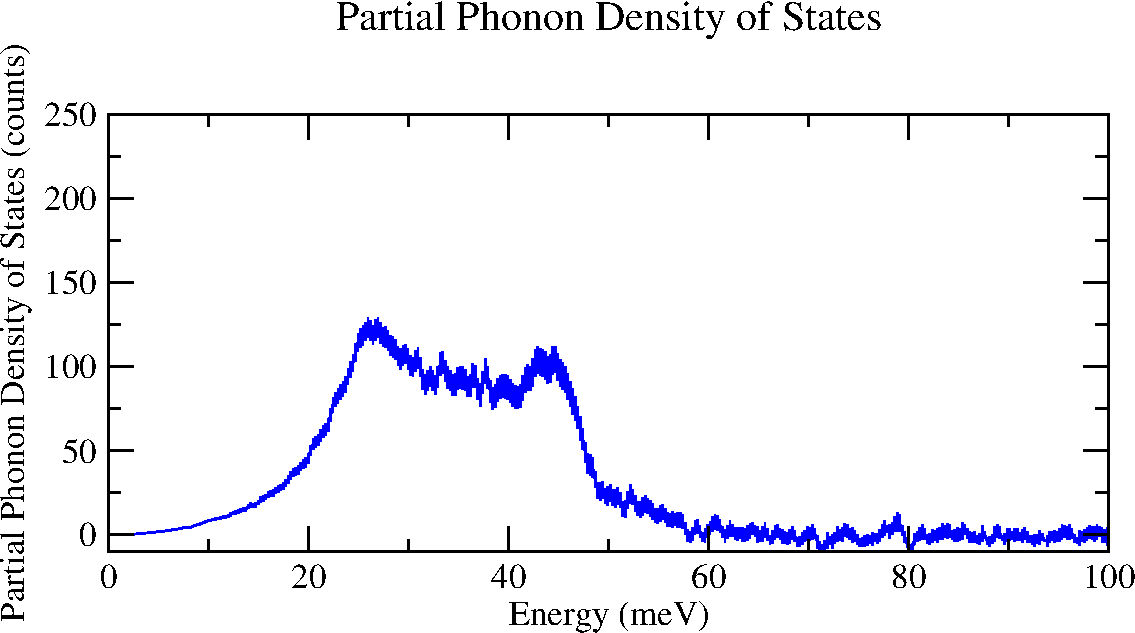
\includegraphics[width=7.5cm]{2014Feb_DAC13_P2//PhoxFigures/PDOS_FeNiSi_DAC13_P2.pdf}} \quad
\subfloat{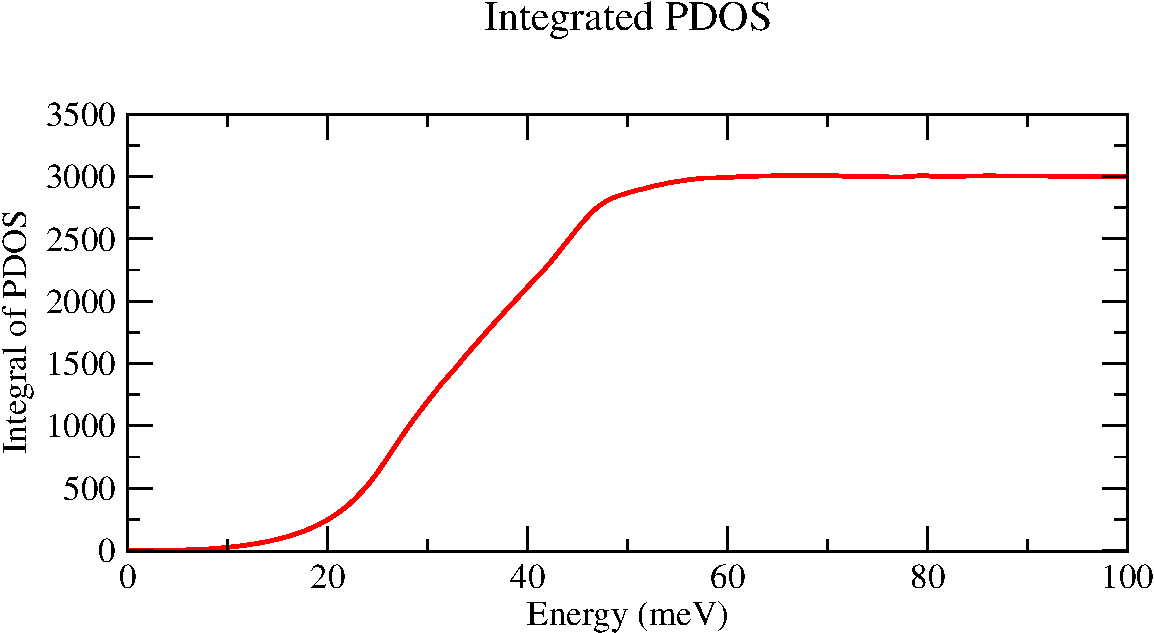
\includegraphics[width=7.5cm]{2014Feb_DAC13_P2//PhoxFigures/IntPDOS_FeNiSi_DAC13_P2.pdf}} \\
\subfloat{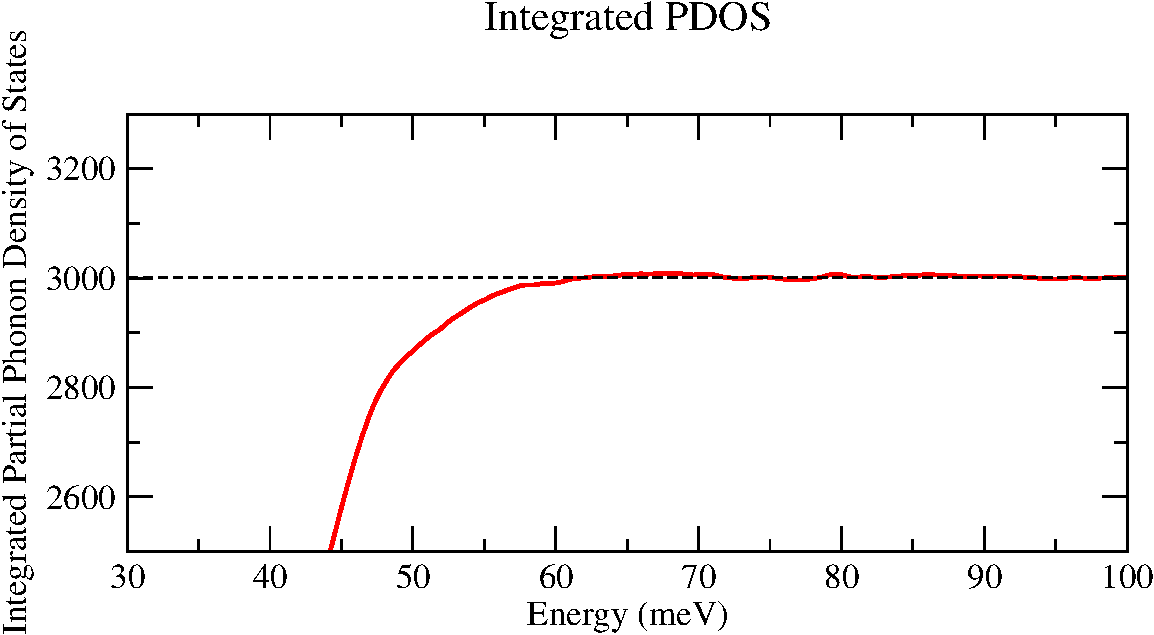
\includegraphics[width=8.0cm]{2014Feb_DAC13_P2//PhoxFigures/IntPDOSZoom_FeNiSi_DAC13_P2.pdf}} \quad
\subfloat{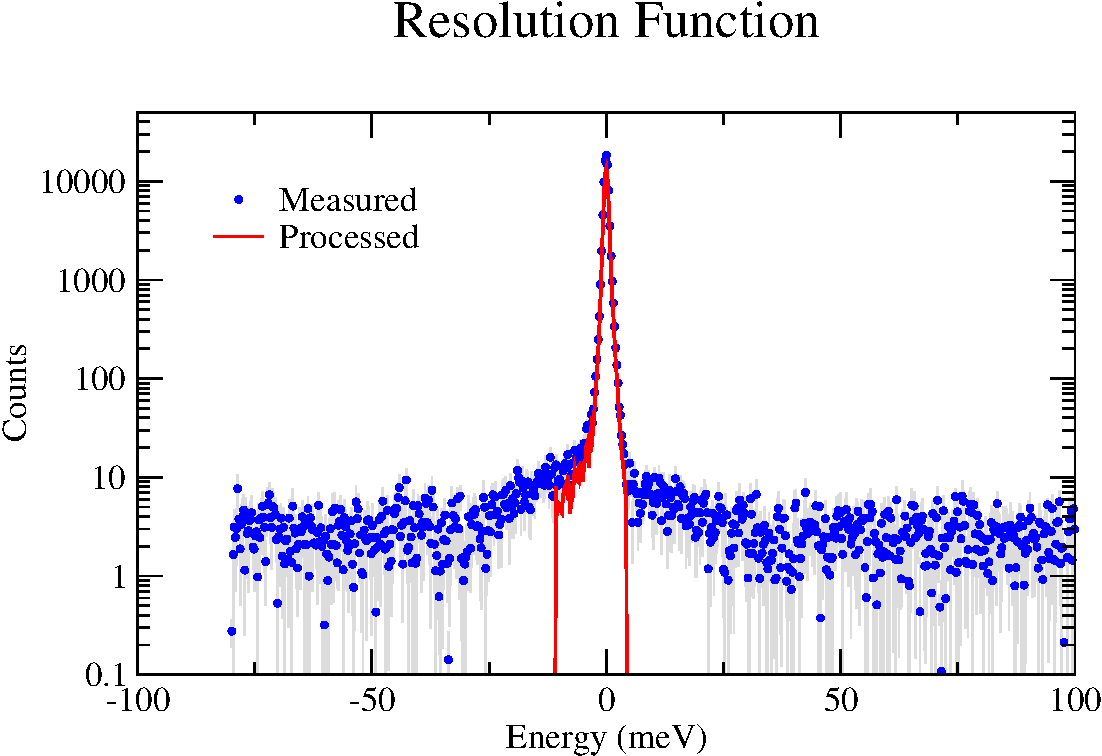
\includegraphics[width=7.5cm]{2014Feb_DAC13_P2//PhoxFigures/ResPeak_FeNiSi_DAC13_P2.pdf}}
\caption{PHOENIX phox data for Fe$_{0.80}$Ni$_{0.10}$Ni$_{0.10}$ data point FeNiSi\_DAC13\_P2.}
\label{fig:cont}
\end{figure}

\begin{figure}[h!]
\centering
\subfloat{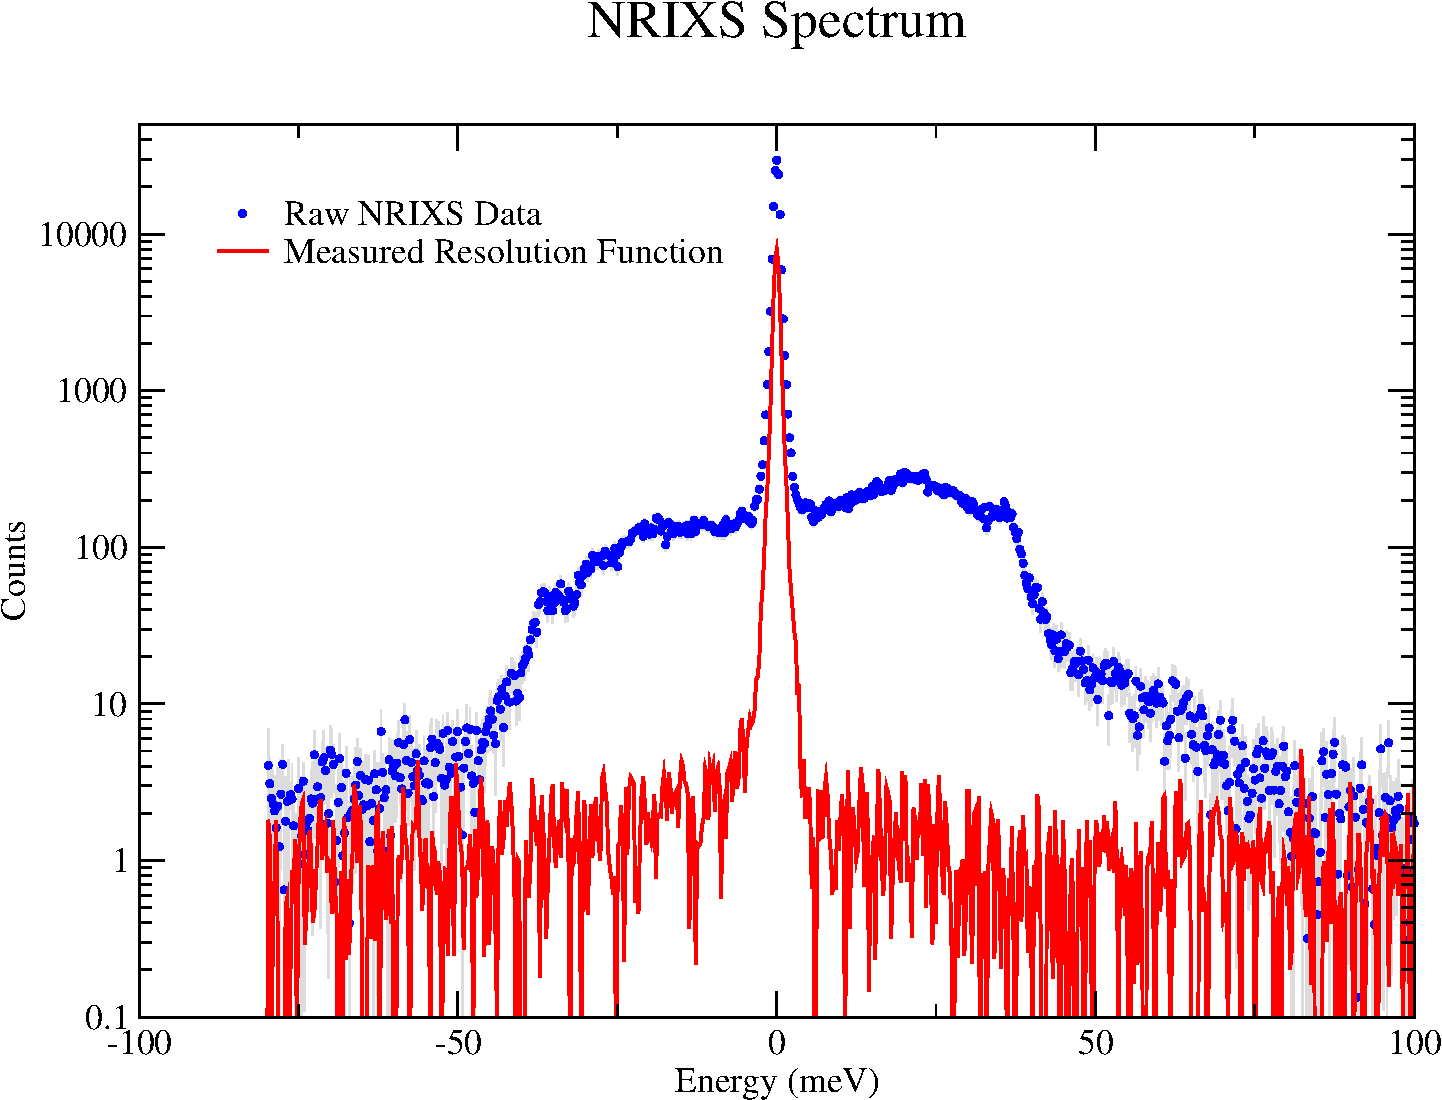
\includegraphics[width=8.0cm]{2014Feb_DAC15_P1//PhoxFigures/NRIXS_FeNiSi_DAC15_P1.pdf}} \quad
\subfloat{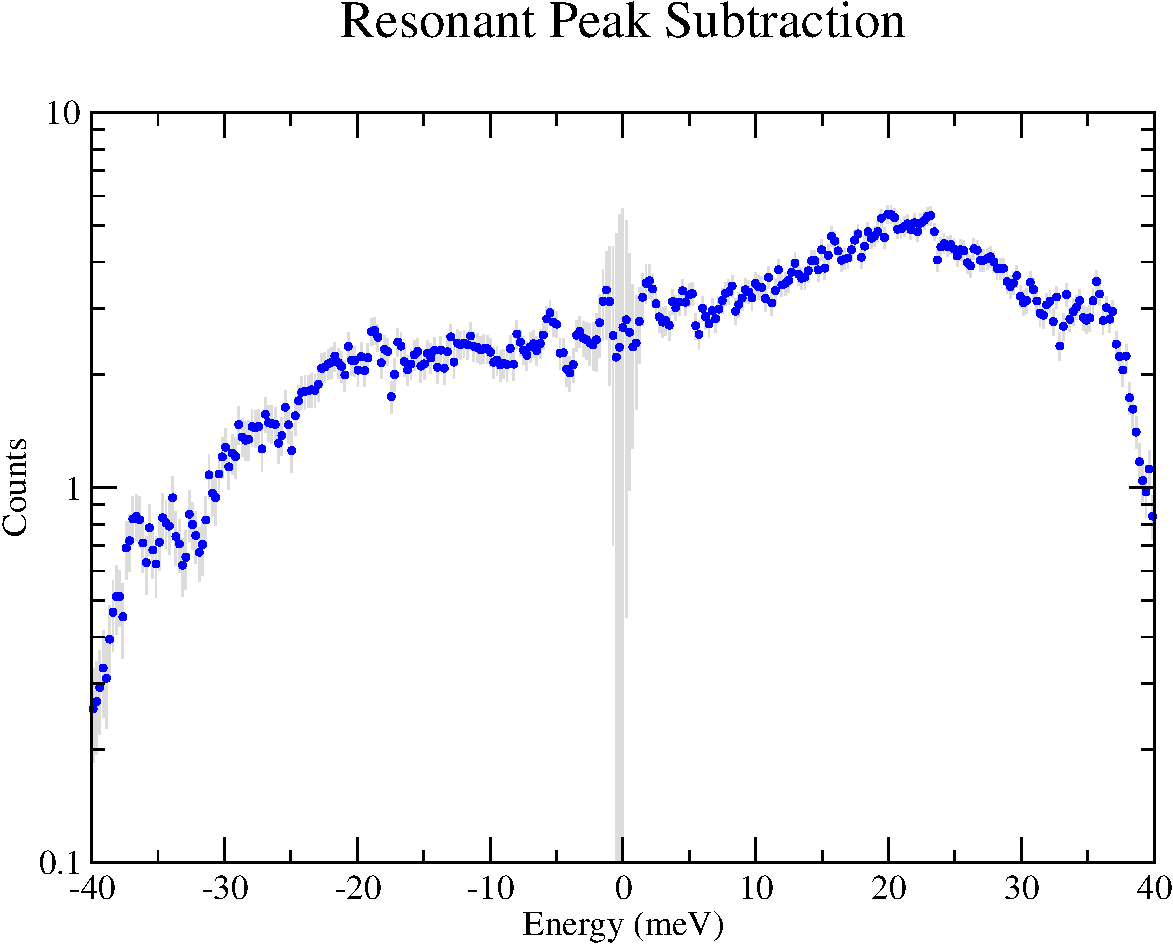
\includegraphics[width=7.5cm]{2014Feb_DAC15_P1//PhoxFigures/PeakSub_FeNiSi_DAC15_P1.pdf}} \\
\subfloat{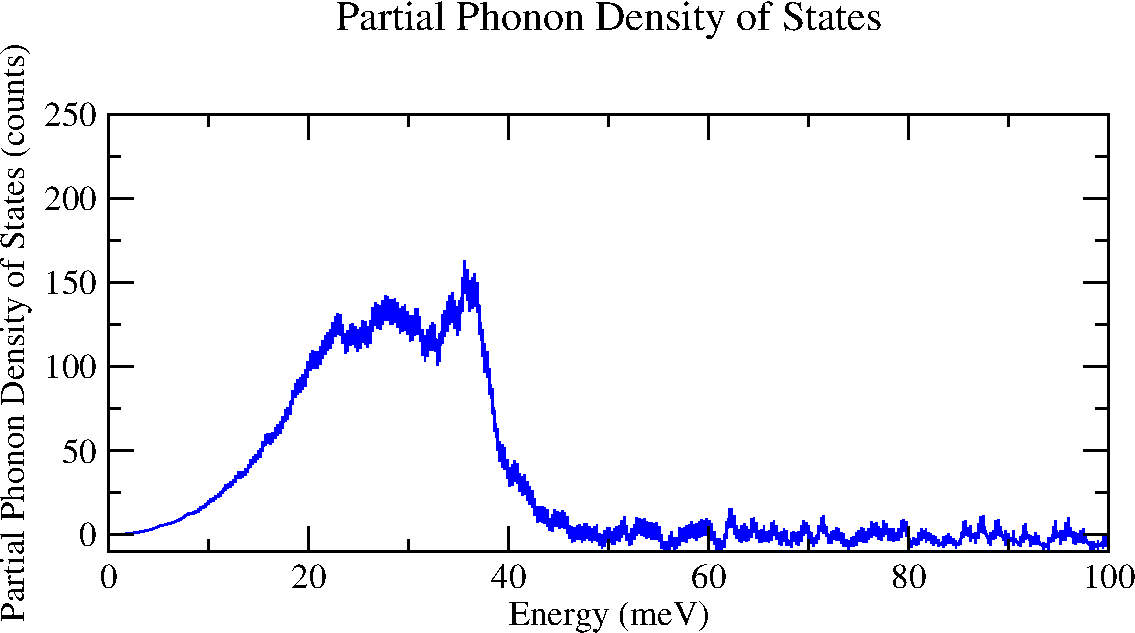
\includegraphics[width=7.5cm]{2014Feb_DAC15_P1//PhoxFigures/PDOS_FeNiSi_DAC15_P1.pdf}} \quad
\subfloat{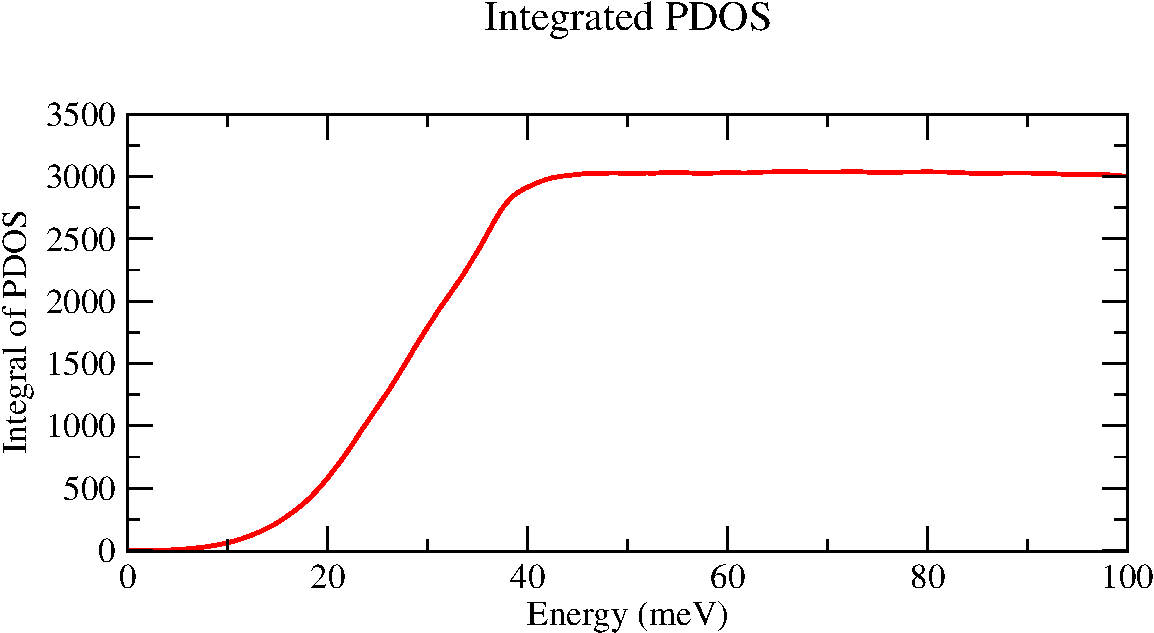
\includegraphics[width=7.5cm]{2014Feb_DAC15_P1//PhoxFigures/IntPDOS_FeNiSi_DAC15_P1.pdf}} \\
\subfloat{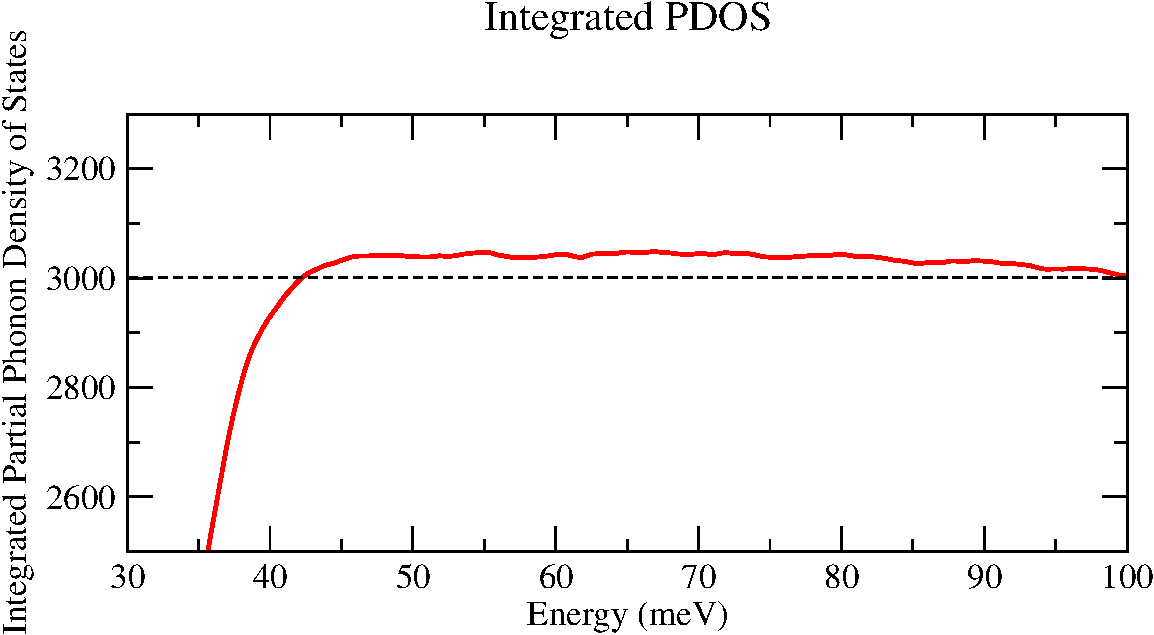
\includegraphics[width=8.0cm]{2014Feb_DAC15_P1//PhoxFigures/IntPDOSZoom_FeNiSi_DAC15_P1.pdf}} \quad
\subfloat{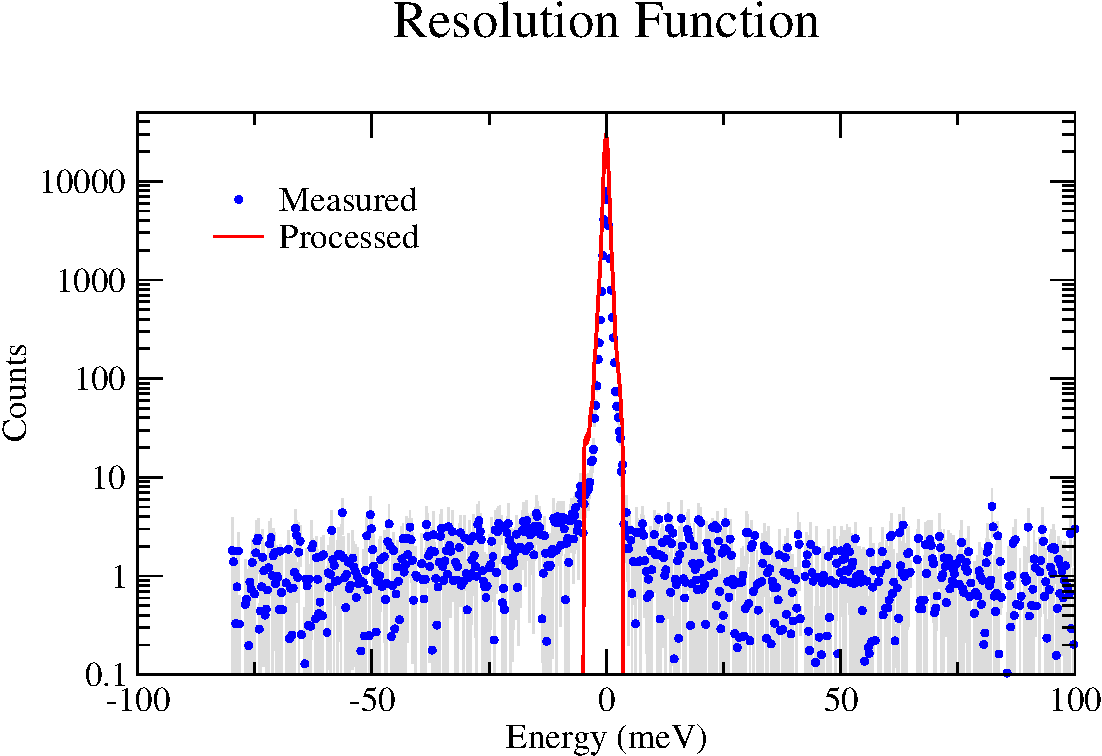
\includegraphics[width=7.5cm]{2014Feb_DAC15_P1//PhoxFigures/ResPeak_FeNiSi_DAC15_P1.pdf}}
\caption{PHOENIX phox data for Fe$_{0.80}$Ni$_{0.10}$Ni$_{0.10}$ data point FeNiSi\_DAC15\_P1.}
\label{fig:cont}
\end{figure}

\begin{figure}[h!]
\centering
\subfloat{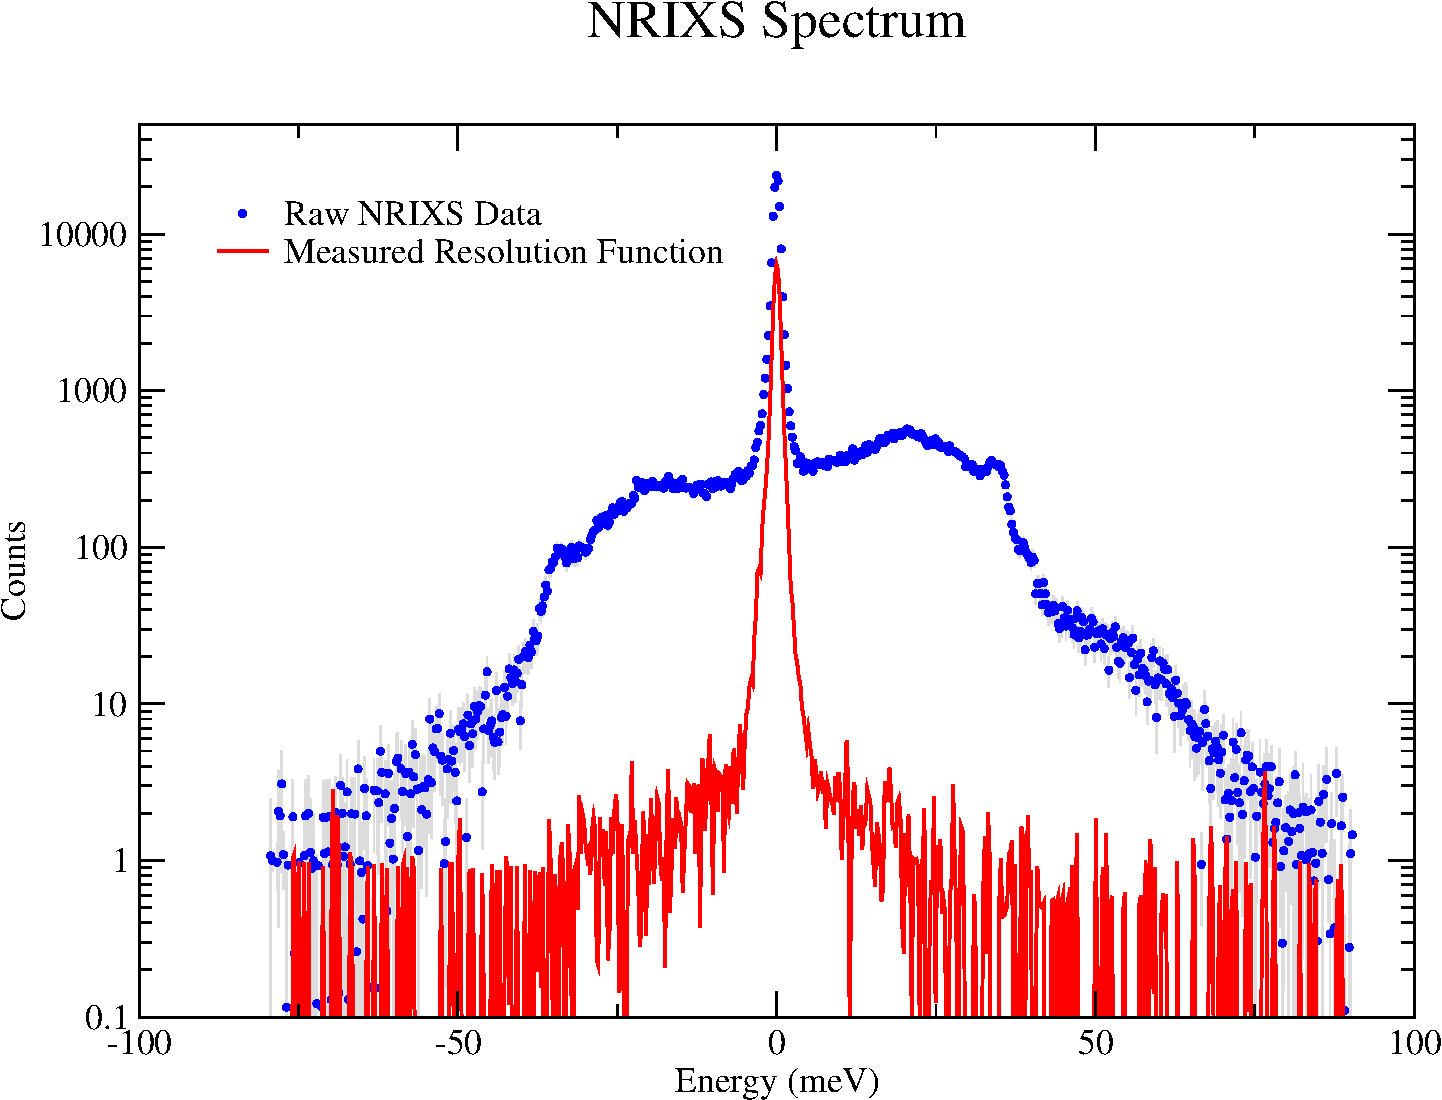
\includegraphics[width=8.0cm]{2015Mar_Ambient//PhoxFigures/NRIXS_FeNiSi_Ambient.pdf}} \quad
\subfloat{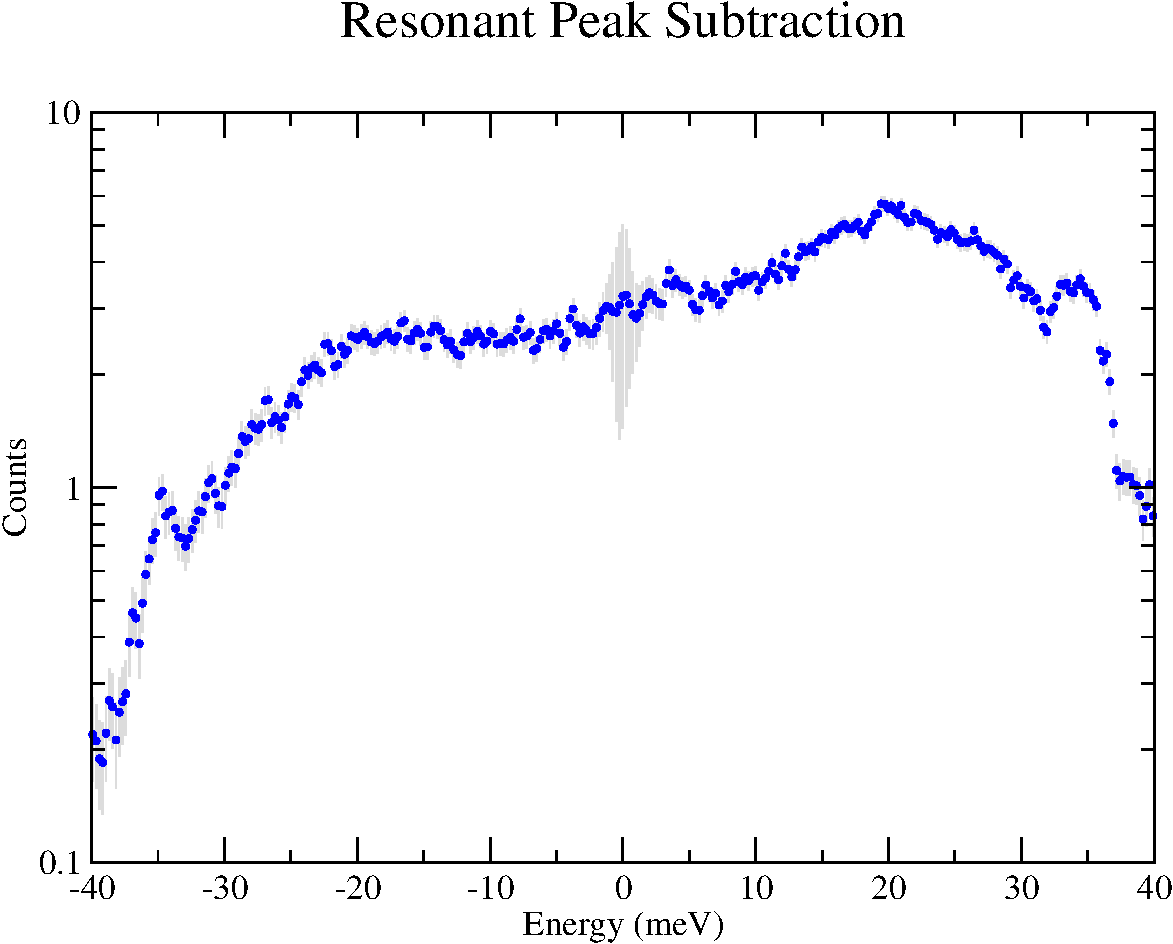
\includegraphics[width=7.5cm]{2015Mar_Ambient//PhoxFigures/PeakSub_FeNiSi_Ambient.pdf}} \\
\subfloat{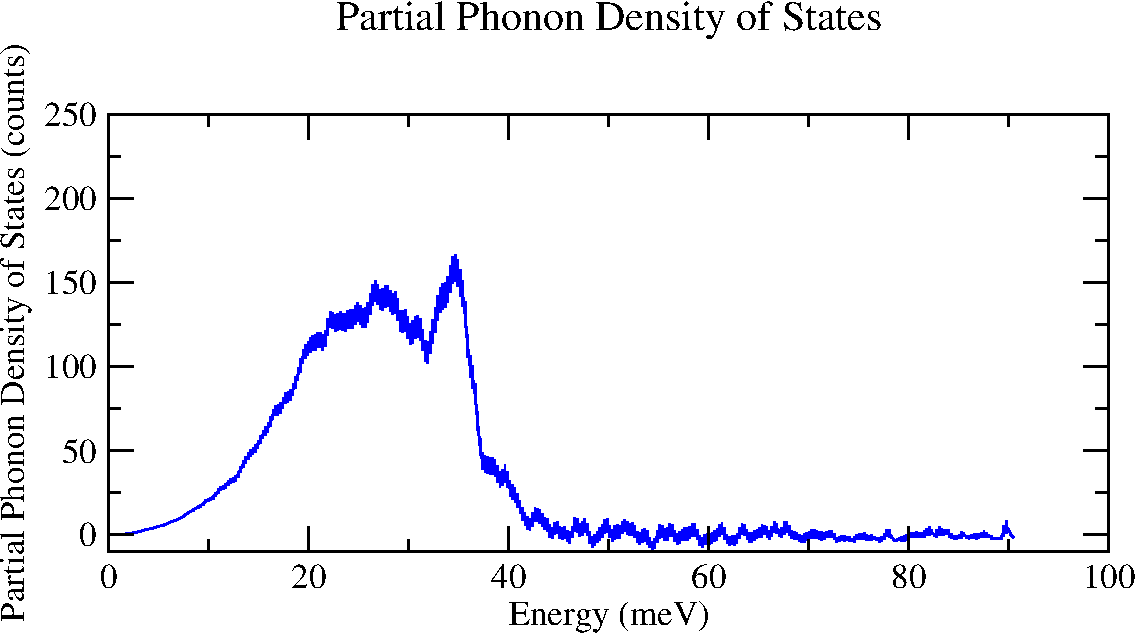
\includegraphics[width=7.5cm]{2015Mar_Ambient//PhoxFigures/PDOS_FeNiSi_Ambient.pdf}} \quad
\subfloat{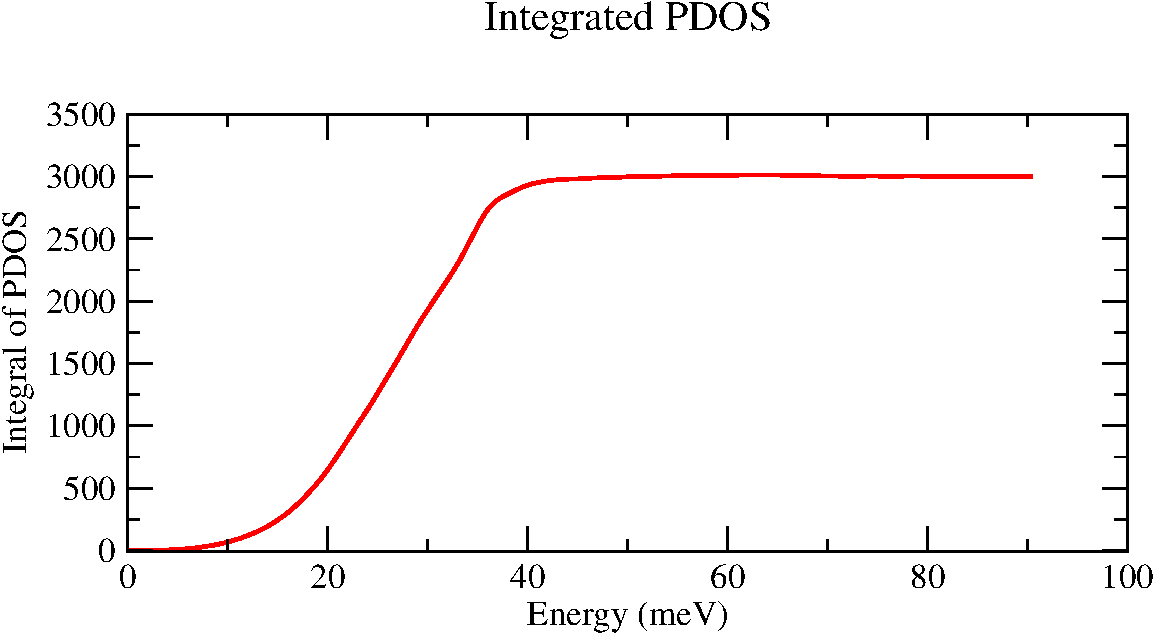
\includegraphics[width=7.5cm]{2015Mar_Ambient//PhoxFigures/IntPDOS_FeNiSi_Ambient.pdf}} \\
\subfloat{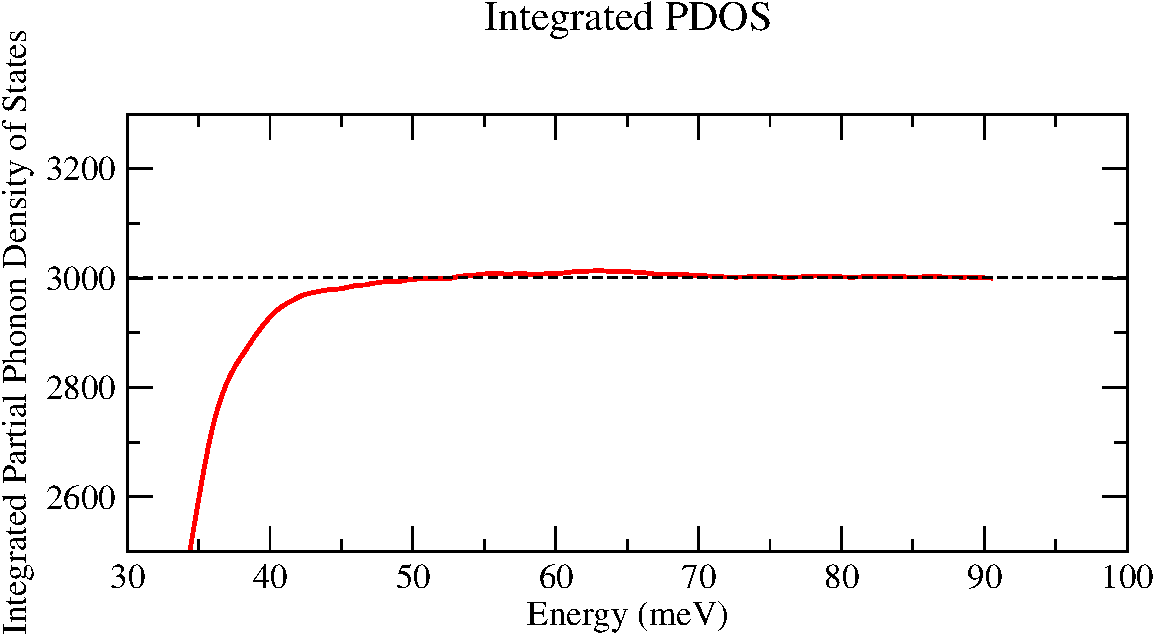
\includegraphics[width=8.0cm]{2015Mar_Ambient//PhoxFigures/IntPDOSZoom_FeNiSi_Ambient.pdf}} \quad
\subfloat{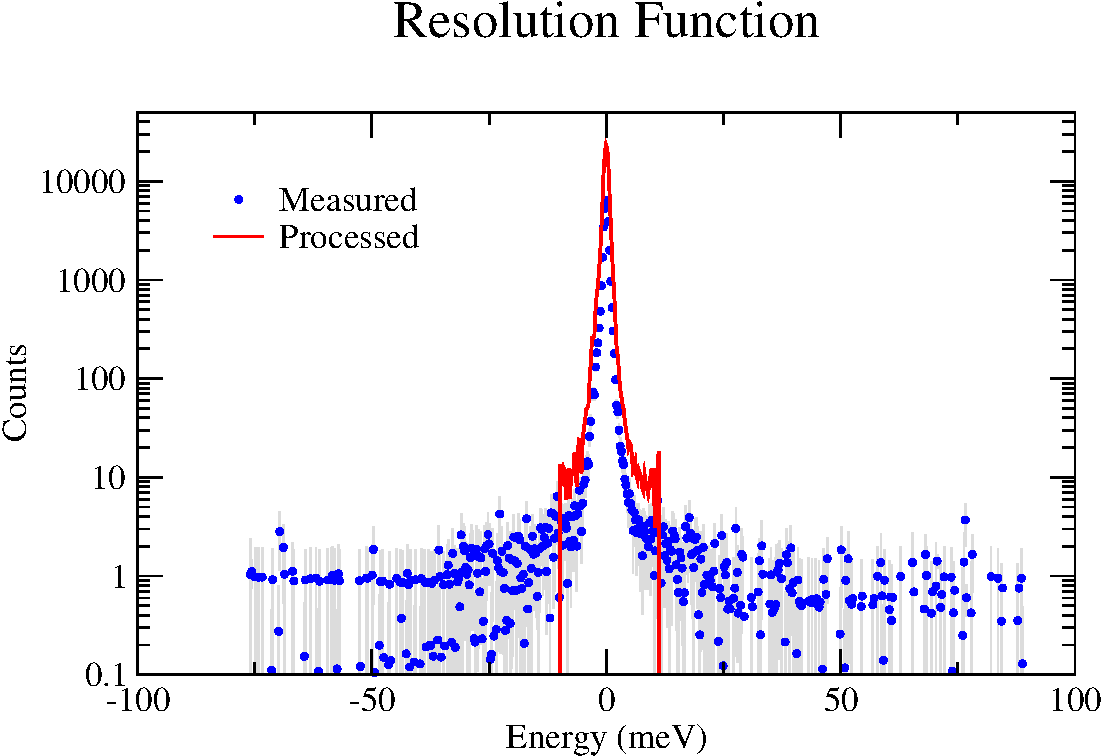
\includegraphics[width=7.5cm]{2015Mar_Ambient//PhoxFigures/ResPeak_FeNiSi_Ambient.pdf}}
\caption{PHOENIX phox data for Fe$_{0.80}$Ni$_{0.10}$Ni$_{0.10}$ data point FeNiSi\_Ambient.}
\label{fig:cont}
\end{figure}

\begin{figure}[h!]
\centering
\subfloat{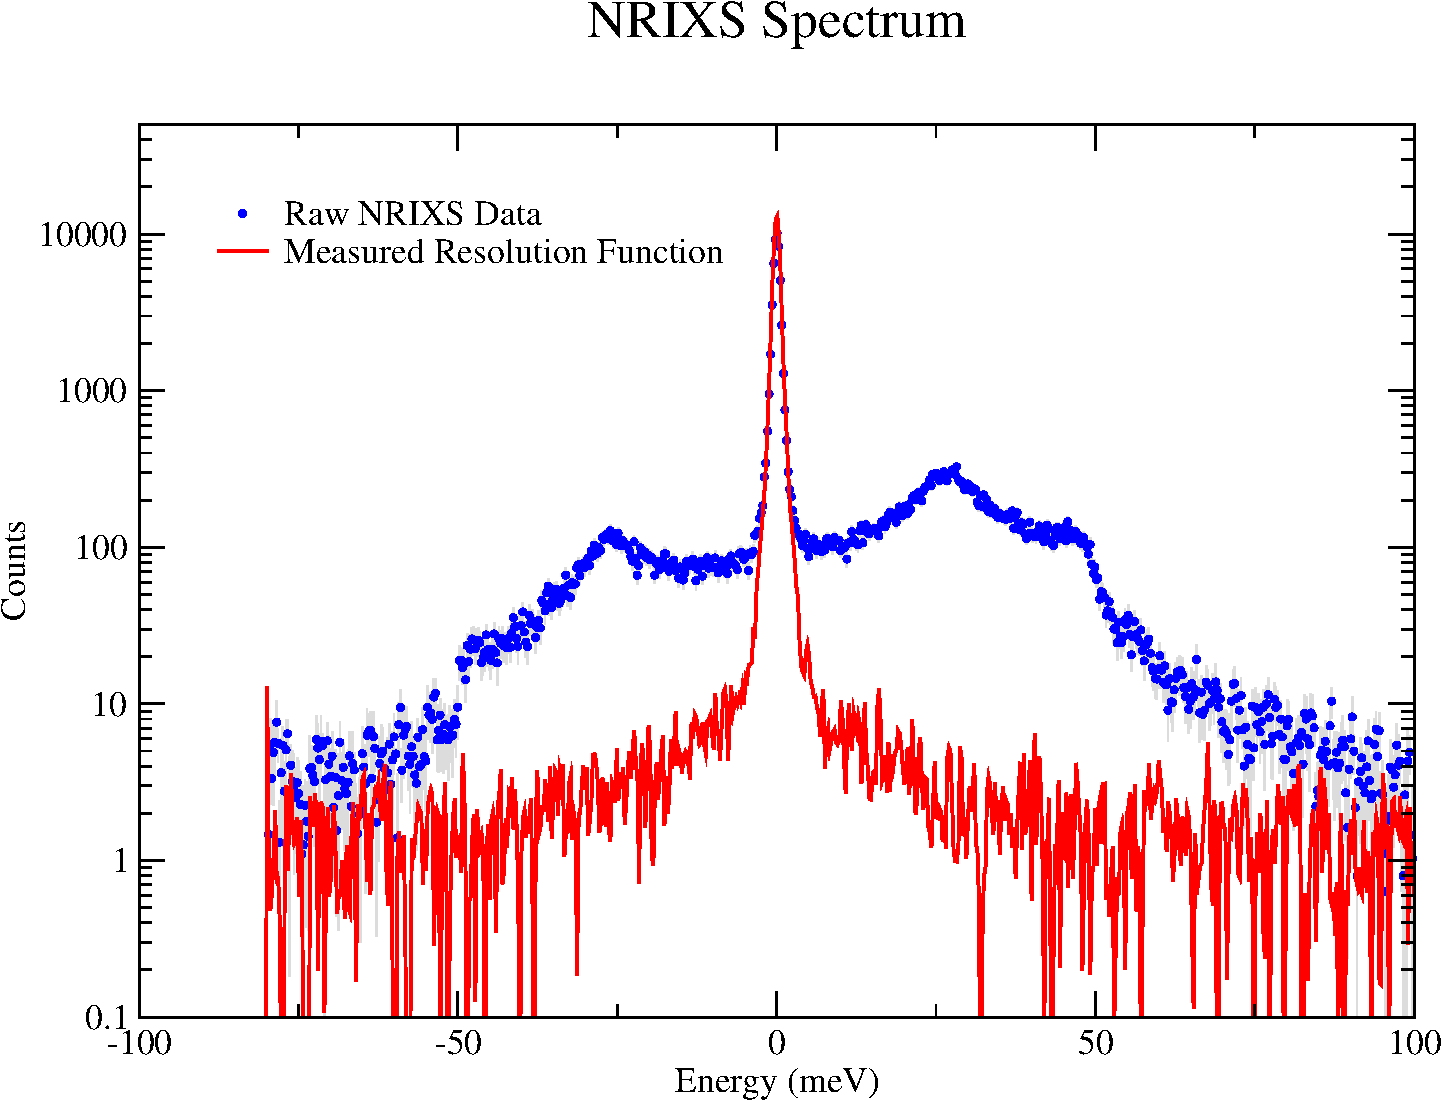
\includegraphics[width=8.0cm]{2015Mar_DAC13_P3//PhoxFigures/NRIXS_FeNiSi_DAC13_P3.pdf}} \quad
\subfloat{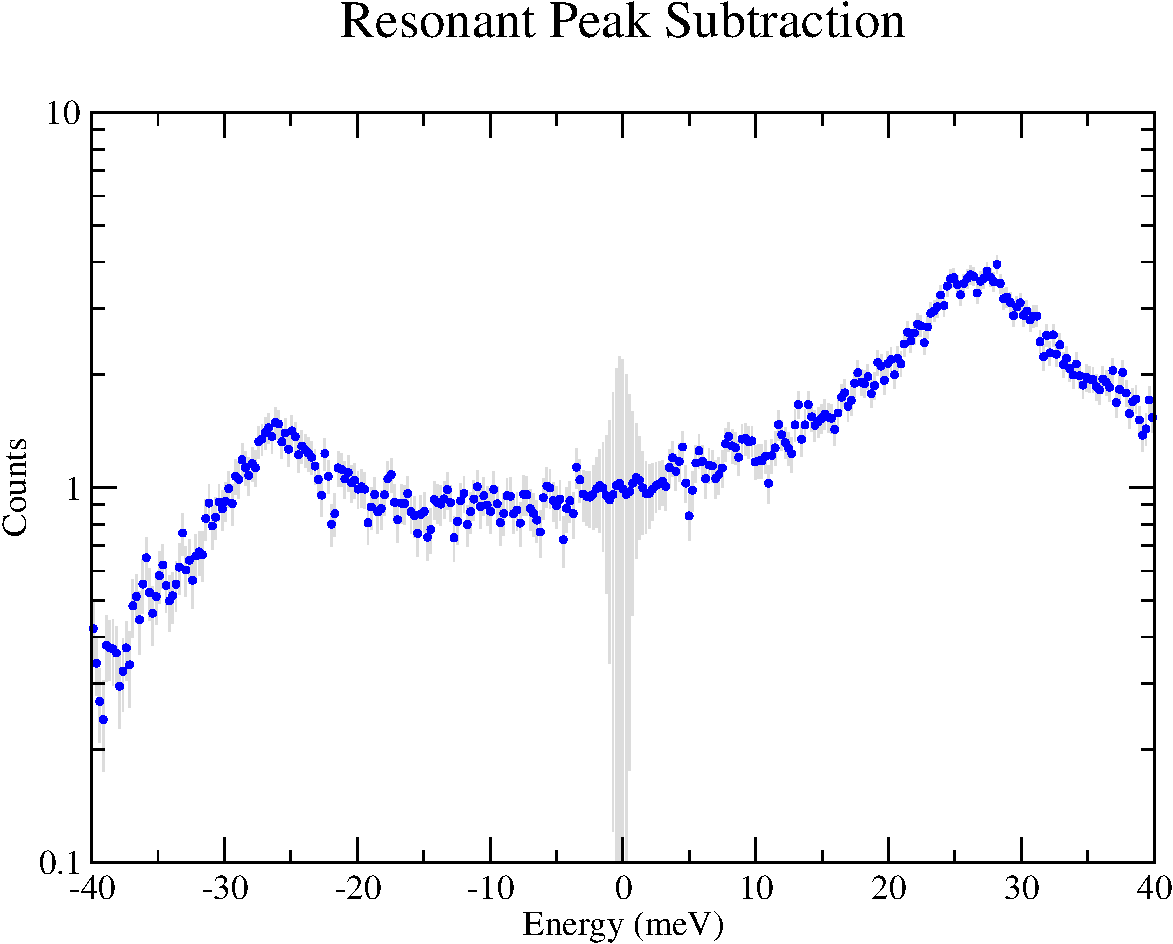
\includegraphics[width=7.5cm]{2015Mar_DAC13_P3//PhoxFigures/PeakSub_FeNiSi_DAC13_P3.pdf}} \\
\subfloat{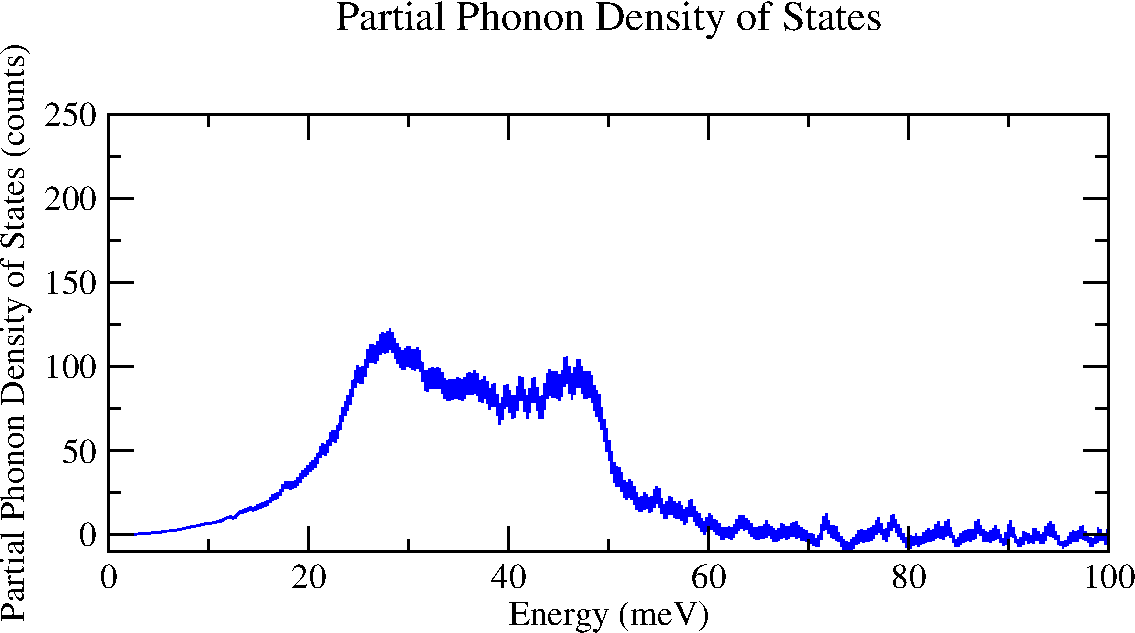
\includegraphics[width=7.5cm]{2015Mar_DAC13_P3//PhoxFigures/PDOS_FeNiSi_DAC13_P3.pdf}} \quad
\subfloat{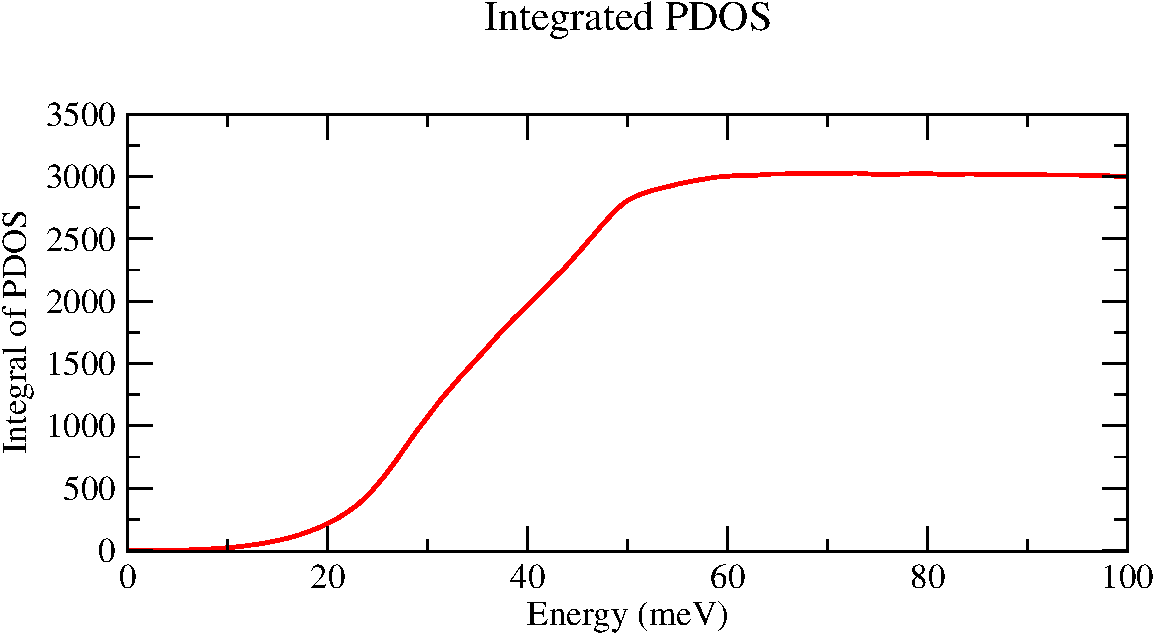
\includegraphics[width=7.5cm]{2015Mar_DAC13_P3//PhoxFigures/IntPDOS_FeNiSi_DAC13_P3.pdf}} \\
\subfloat{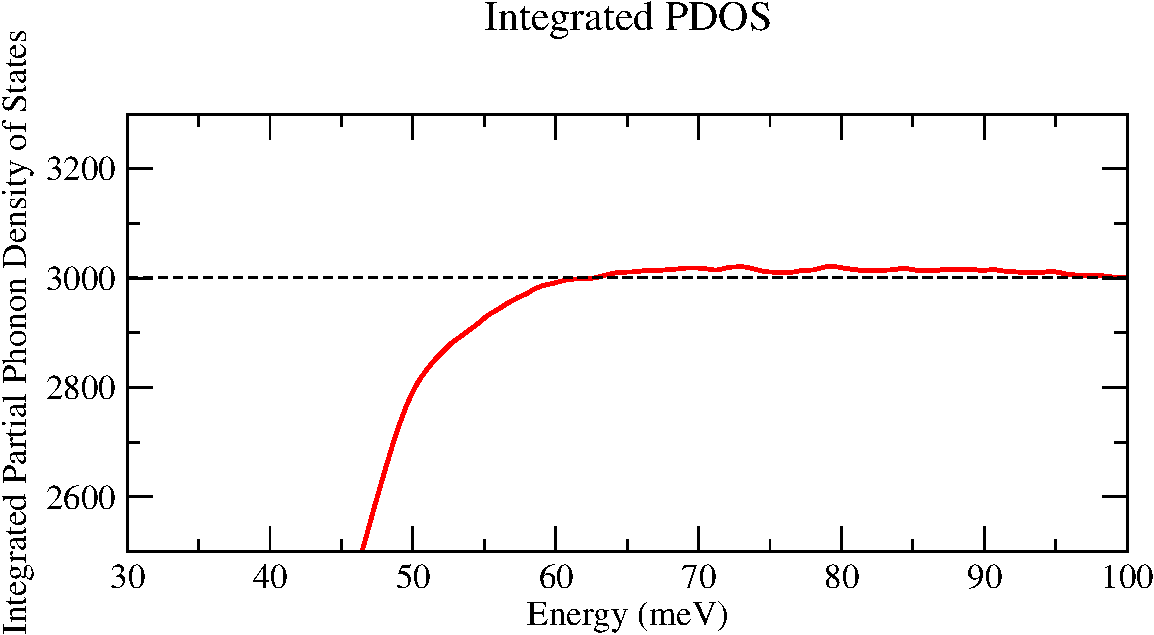
\includegraphics[width=8.0cm]{2015Mar_DAC13_P3//PhoxFigures/IntPDOSZoom_FeNiSi_DAC13_P3.pdf}} \quad
\subfloat{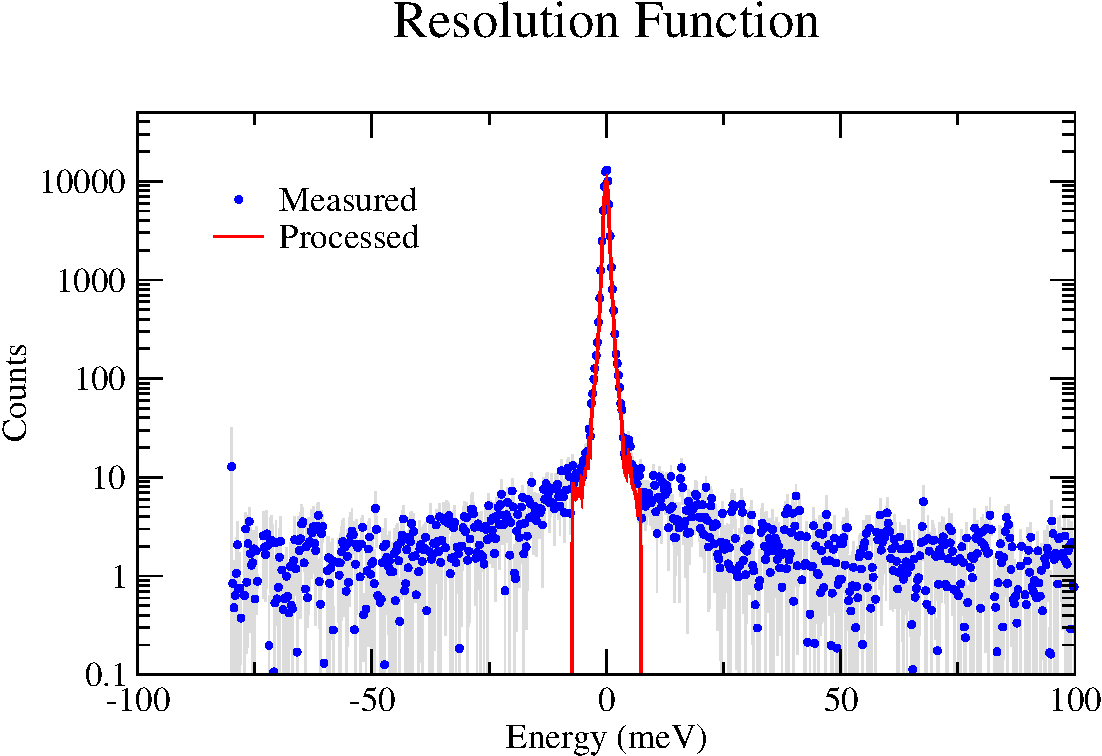
\includegraphics[width=7.5cm]{2015Mar_DAC13_P3//PhoxFigures/ResPeak_FeNiSi_DAC13_P3.pdf}}
\caption{PHOENIX phox data for Fe$_{0.80}$Ni$_{0.10}$Ni$_{0.10}$ data point FeNiSi\_DAC13\_P3.}
\label{fig:cont}
\end{figure}

\begin{figure}[h!]
\centering
\subfloat{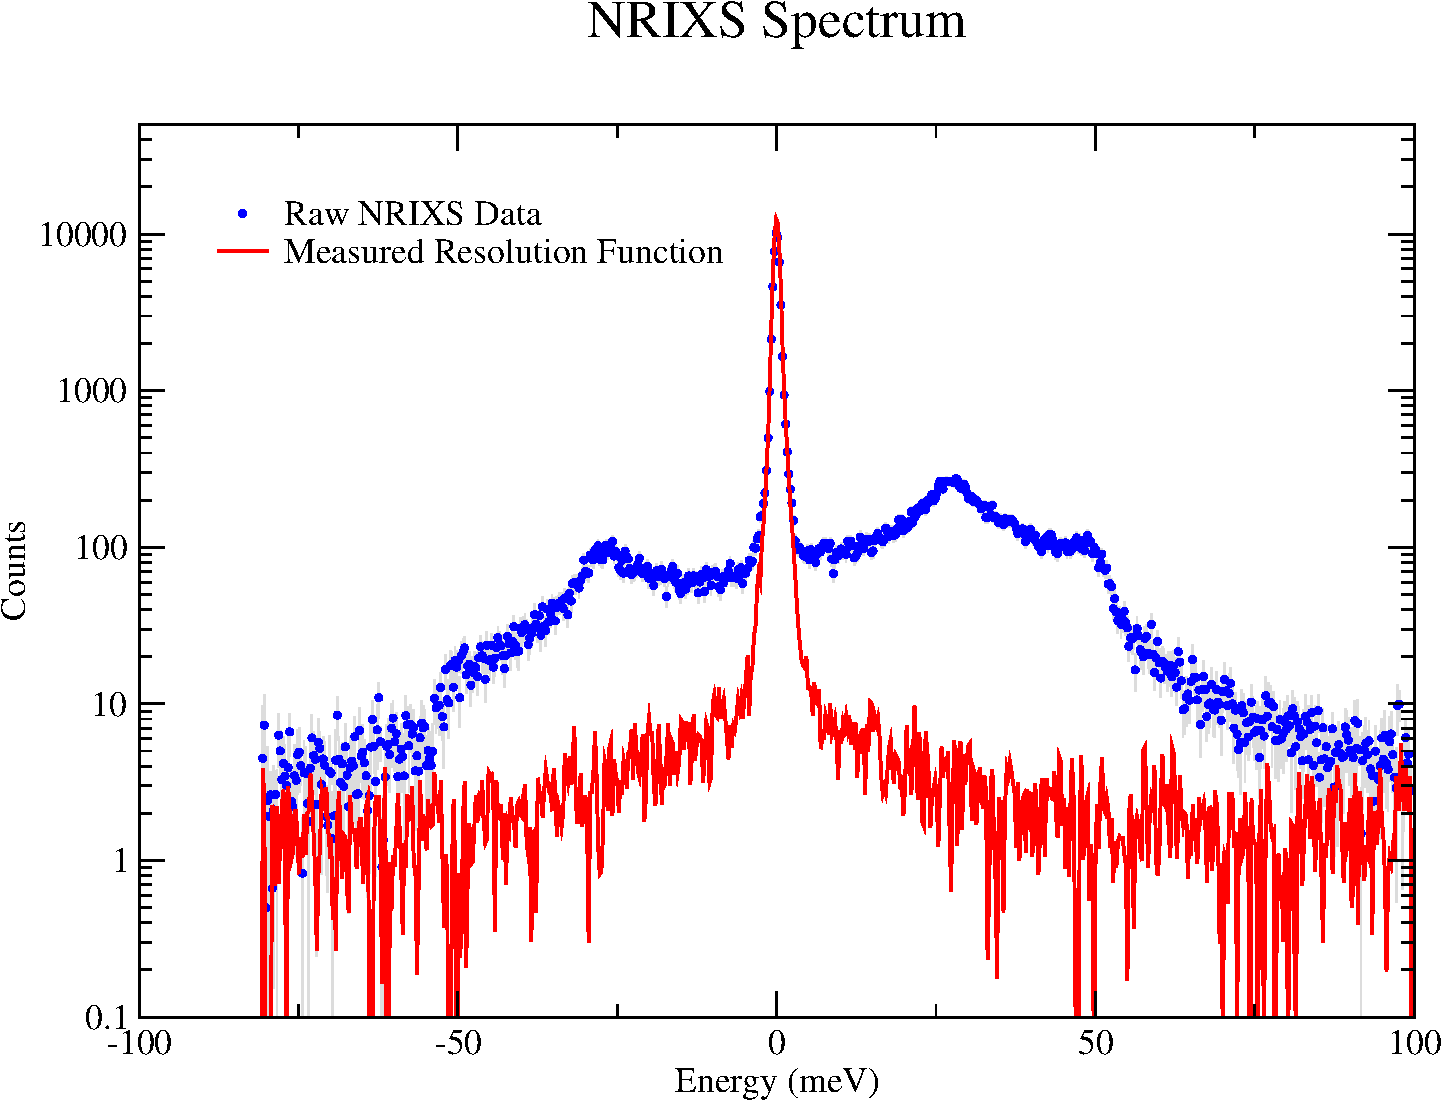
\includegraphics[width=8.0cm]{2015Mar_DAC13_P4//PhoxFigures/NRIXS_FeNiSi_DAC13_P4.pdf}} \quad
\subfloat{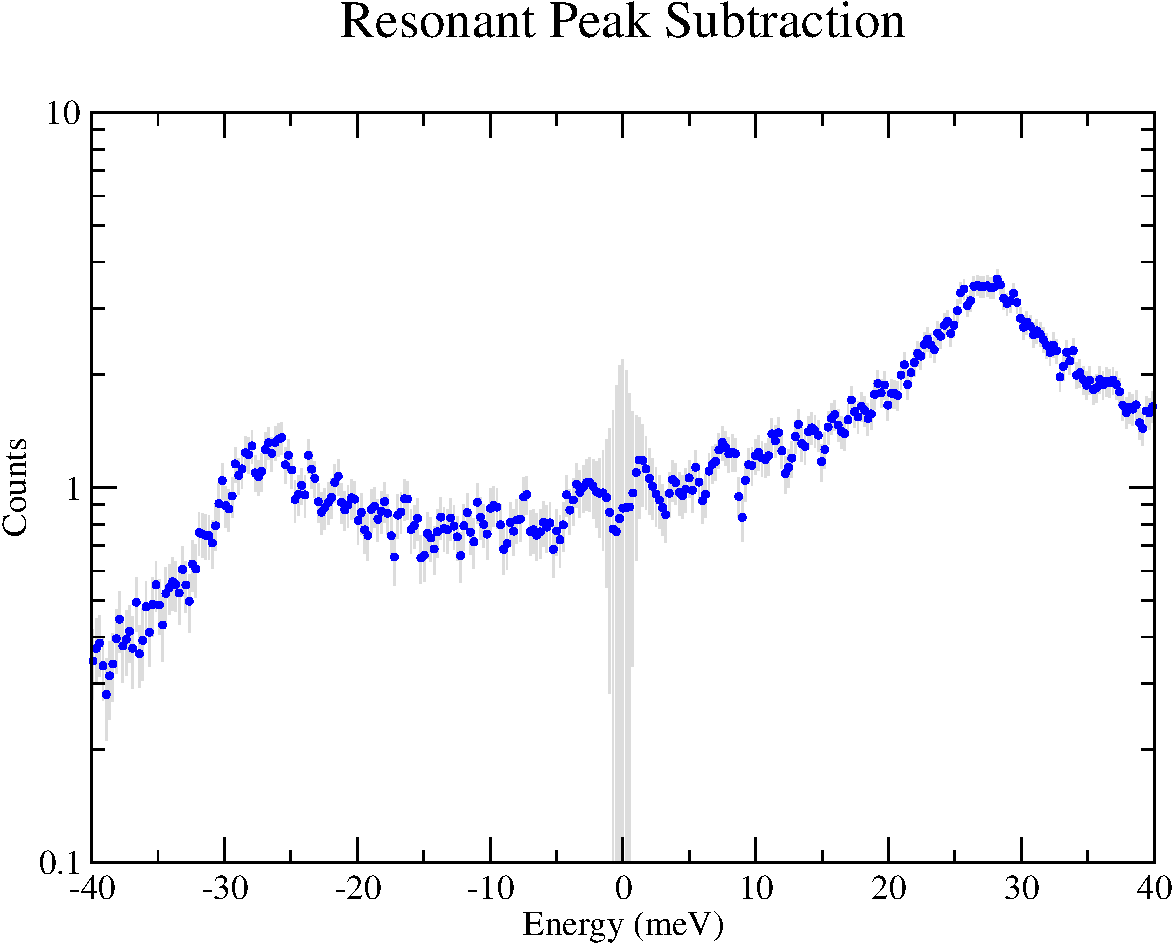
\includegraphics[width=7.5cm]{2015Mar_DAC13_P4//PhoxFigures/PeakSub_FeNiSi_DAC13_P4.pdf}} \\
\subfloat{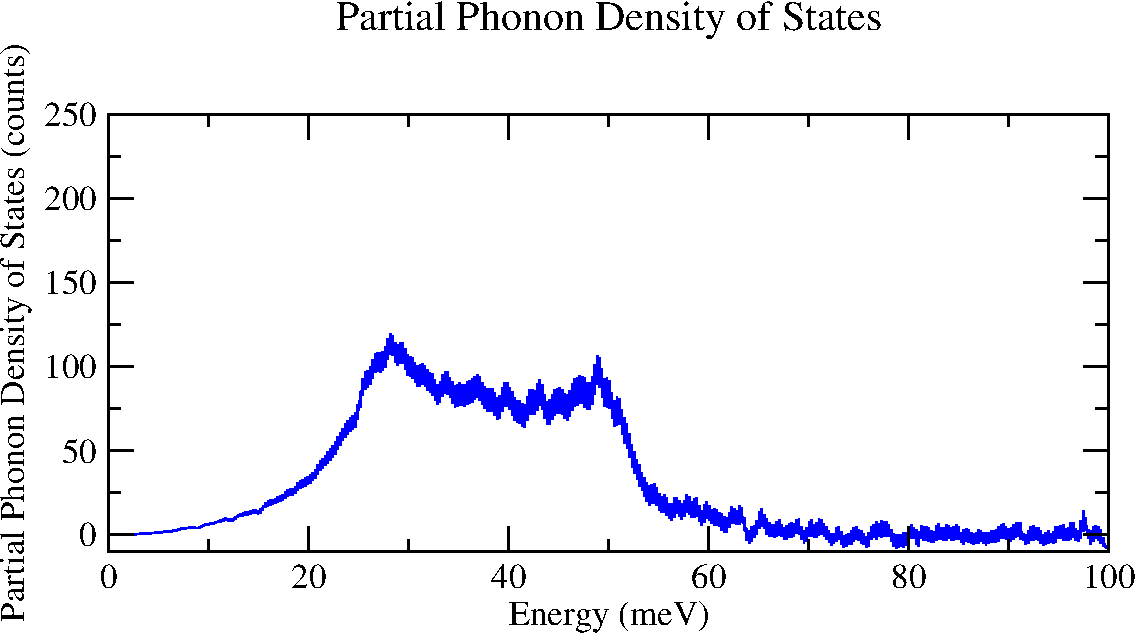
\includegraphics[width=7.5cm]{2015Mar_DAC13_P4//PhoxFigures/PDOS_FeNiSi_DAC13_P4.pdf}} \quad
\subfloat{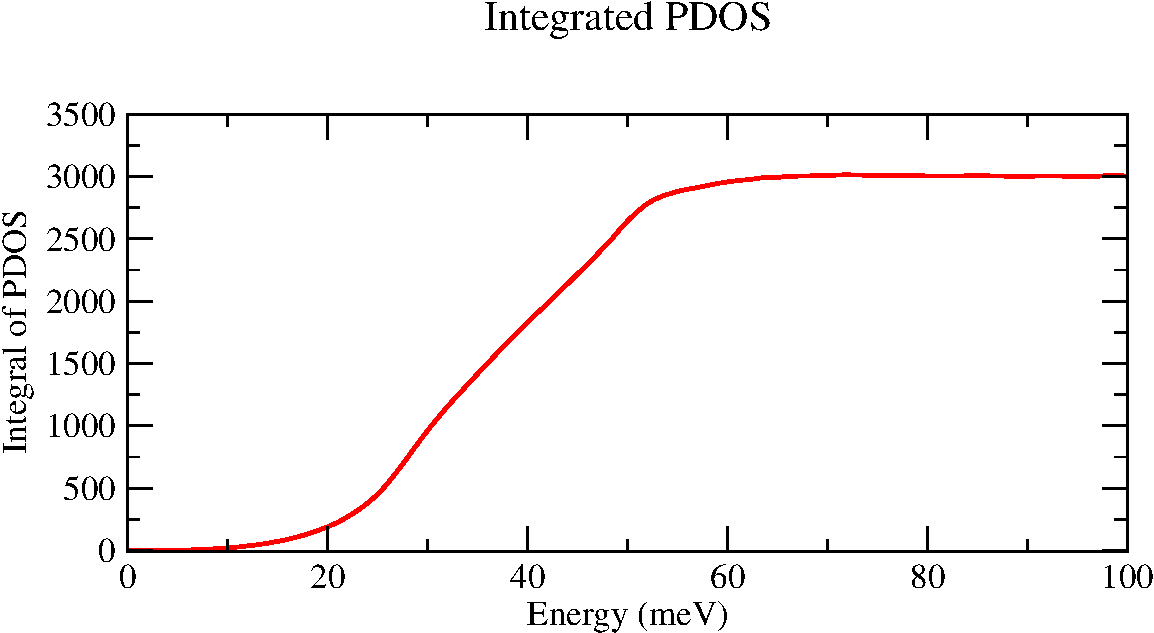
\includegraphics[width=7.5cm]{2015Mar_DAC13_P4//PhoxFigures/IntPDOS_FeNiSi_DAC13_P4.pdf}} \\
\subfloat{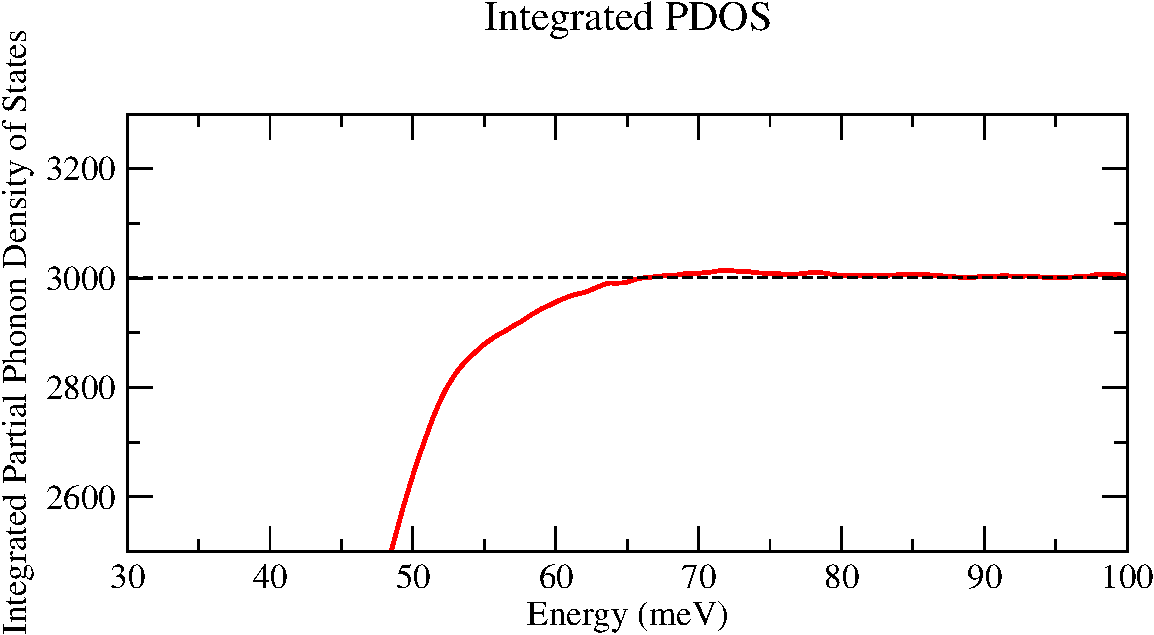
\includegraphics[width=8.0cm]{2015Mar_DAC13_P4//PhoxFigures/IntPDOSZoom_FeNiSi_DAC13_P4.pdf}} \quad
\subfloat{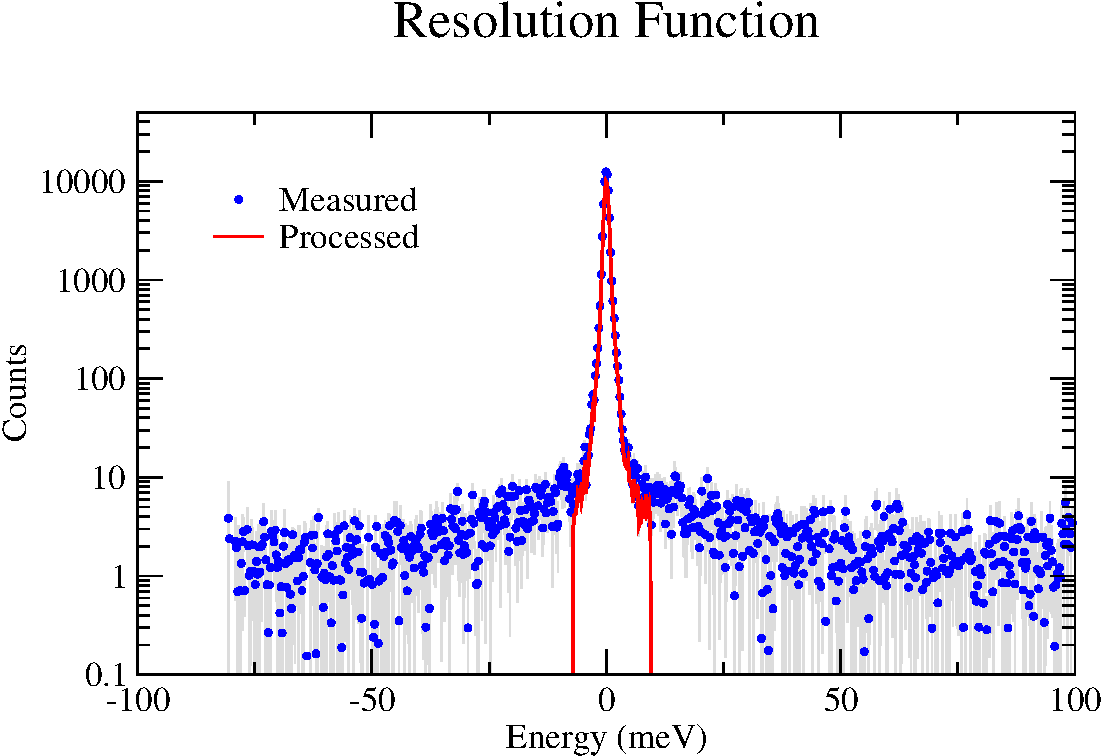
\includegraphics[width=7.5cm]{2015Mar_DAC13_P4//PhoxFigures/ResPeak_FeNiSi_DAC13_P4.pdf}}
\caption{PHOENIX phox data for Fe$_{0.80}$Ni$_{0.10}$Ni$_{0.10}$ data point FeNiSi\_DAC13\_P4.}
\label{fig:cont}
\end{figure}

\begin{figure}[h!]
\centering
\subfloat{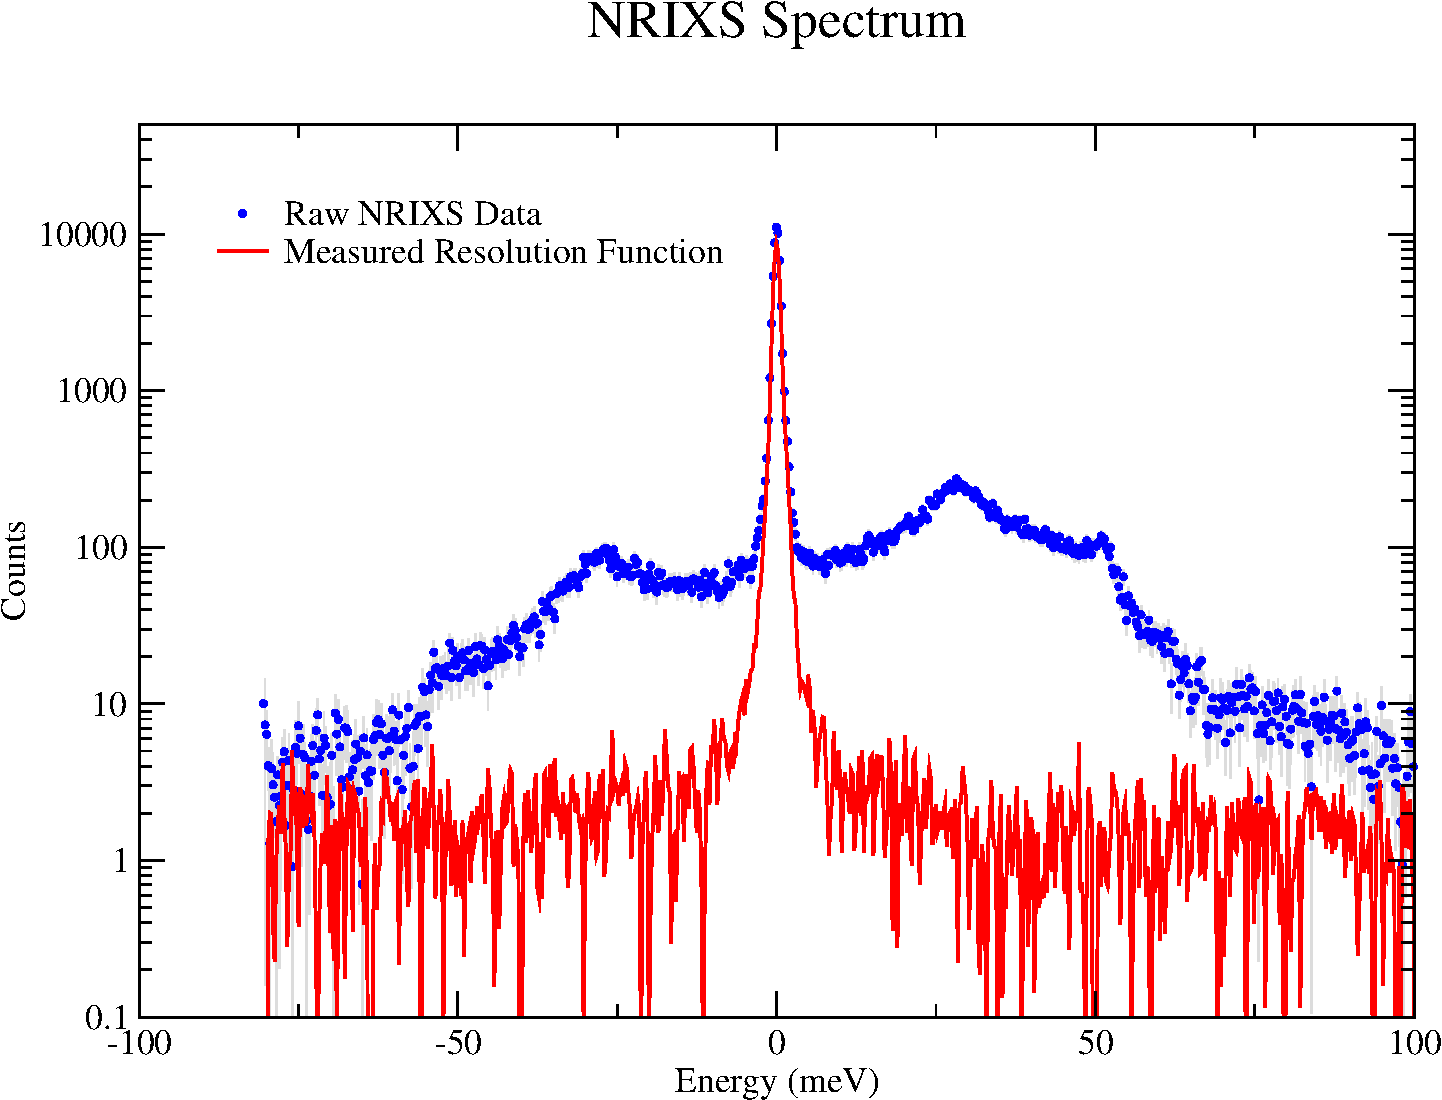
\includegraphics[width=8.0cm]{2015Mar_DAC13_P5//PhoxFigures/NRIXS_FeNiSi_DAC13_P5.pdf}} \quad
\subfloat{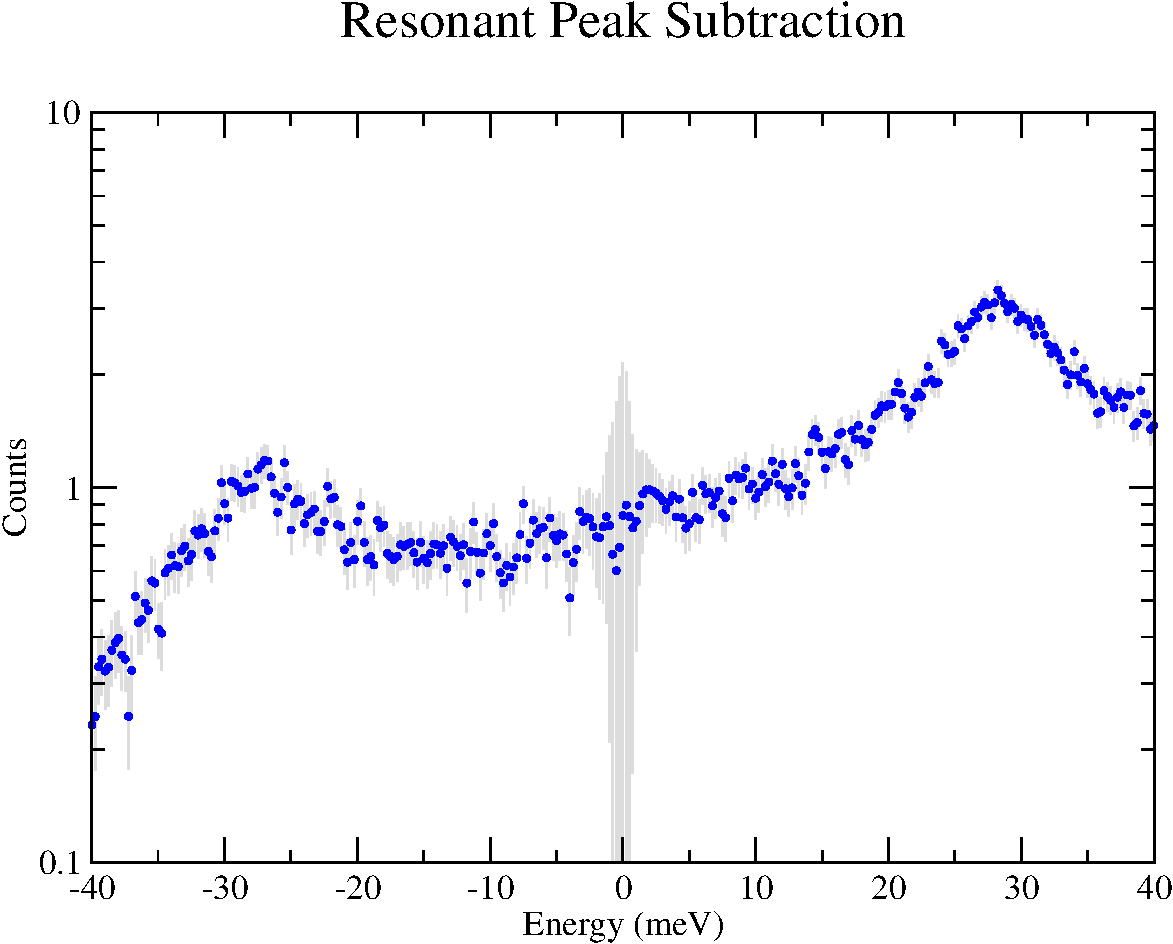
\includegraphics[width=7.5cm]{2015Mar_DAC13_P5//PhoxFigures/PeakSub_FeNiSi_DAC13_P5.pdf}} \\
\subfloat{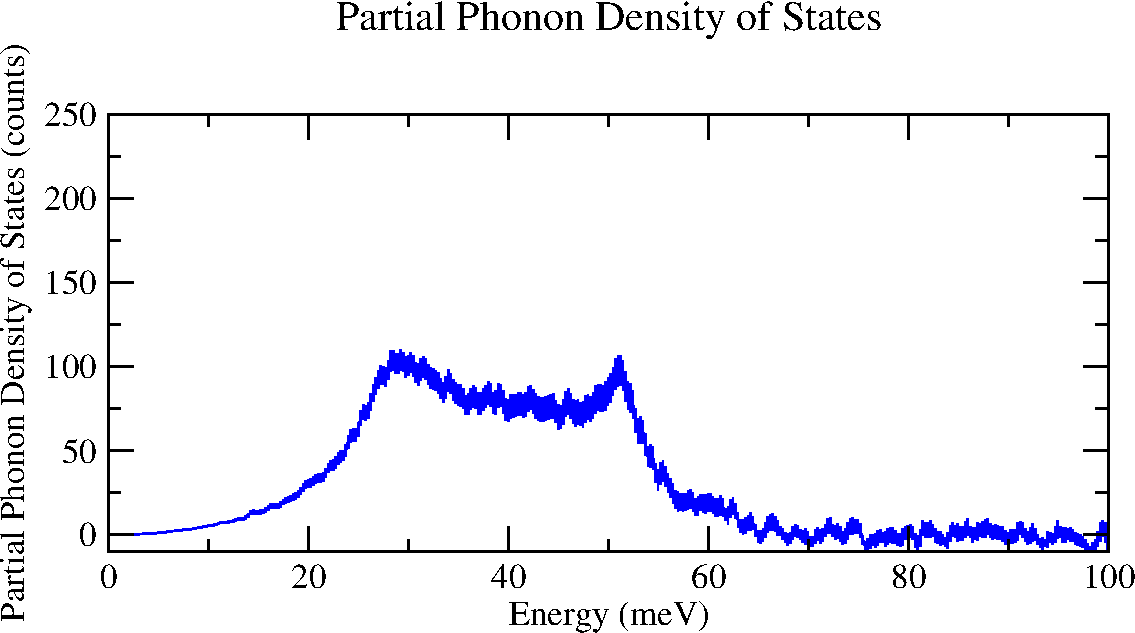
\includegraphics[width=7.5cm]{2015Mar_DAC13_P5//PhoxFigures/PDOS_FeNiSi_DAC13_P5.pdf}} \quad
\subfloat{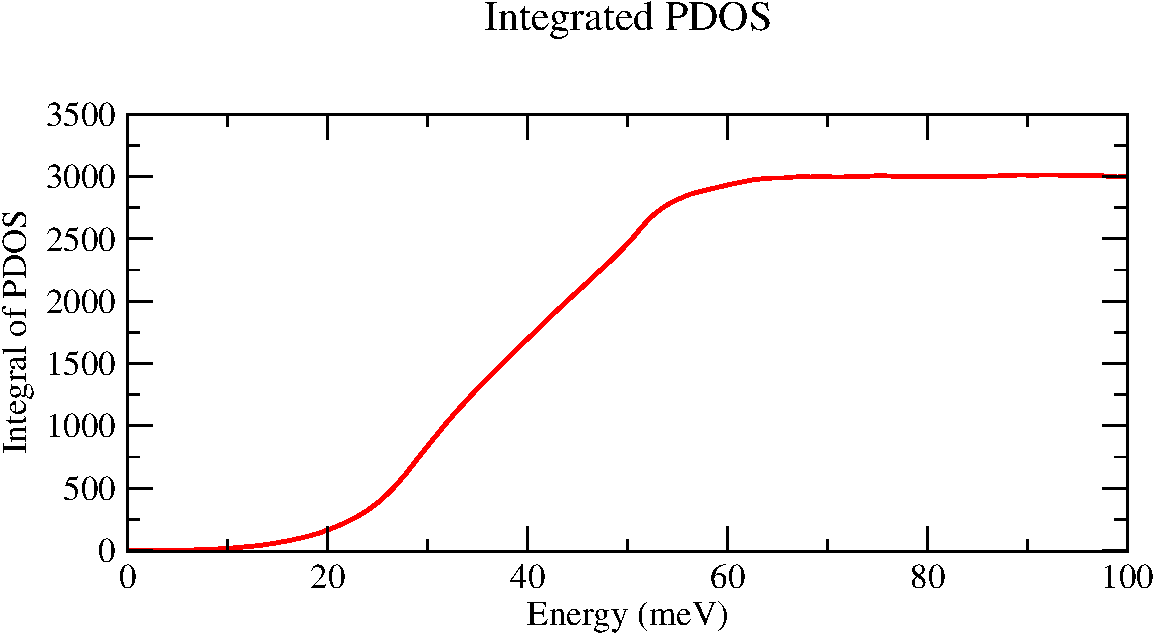
\includegraphics[width=7.5cm]{2015Mar_DAC13_P5//PhoxFigures/IntPDOS_FeNiSi_DAC13_P5.pdf}} \\
\subfloat{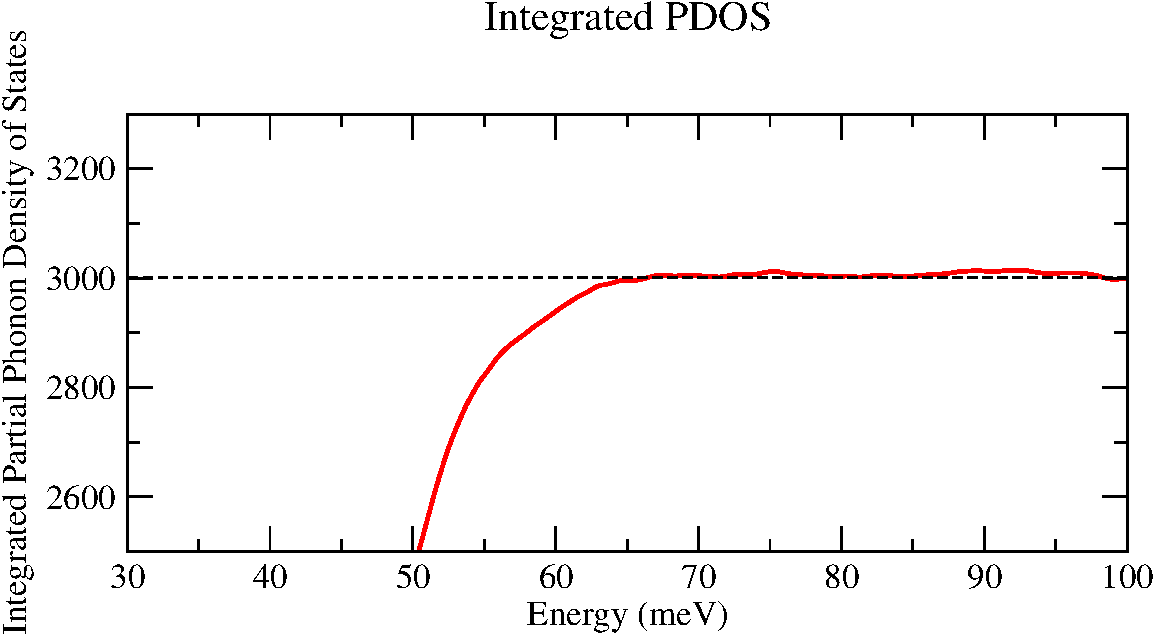
\includegraphics[width=8.0cm]{2015Mar_DAC13_P5//PhoxFigures/IntPDOSZoom_FeNiSi_DAC13_P5.pdf}} \quad
\subfloat{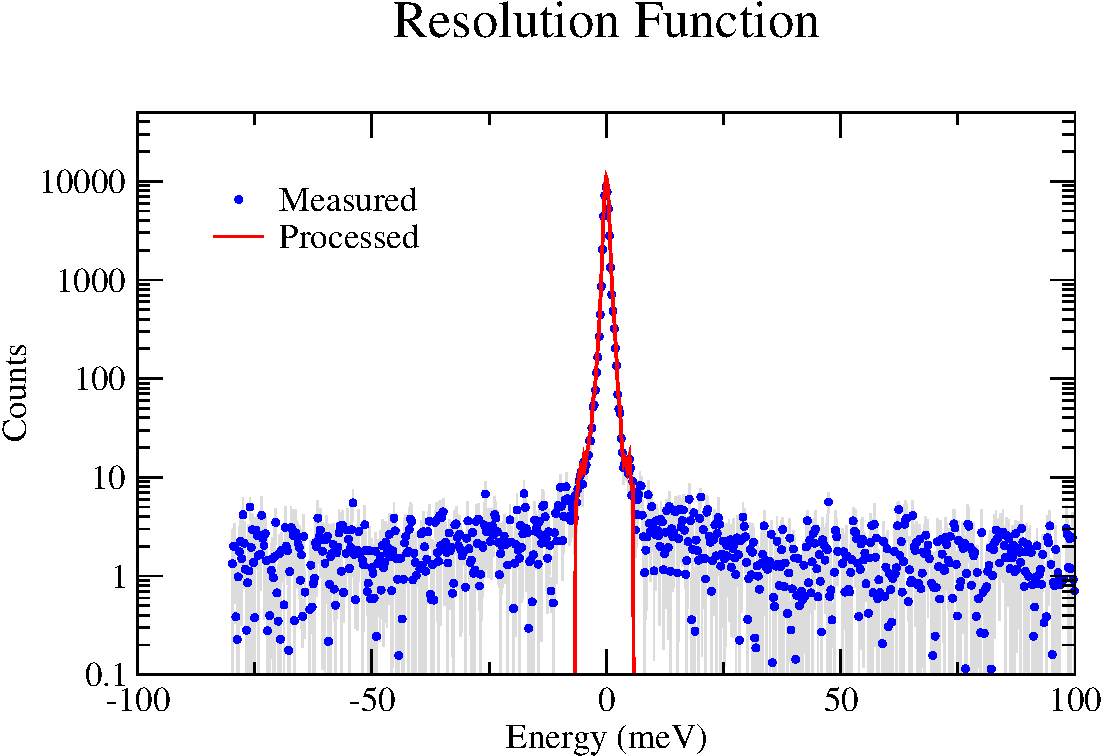
\includegraphics[width=7.5cm]{2015Mar_DAC13_P5//PhoxFigures/ResPeak_FeNiSi_DAC13_P5.pdf}}
\caption{PHOENIX phox data for Fe$_{0.80}$Ni$_{0.10}$Ni$_{0.10}$ data point FeNiSi\_DAC13\_P5.}
\label{fig:cont}
\end{figure}

\begin{figure}[h!]
\centering
\subfloat{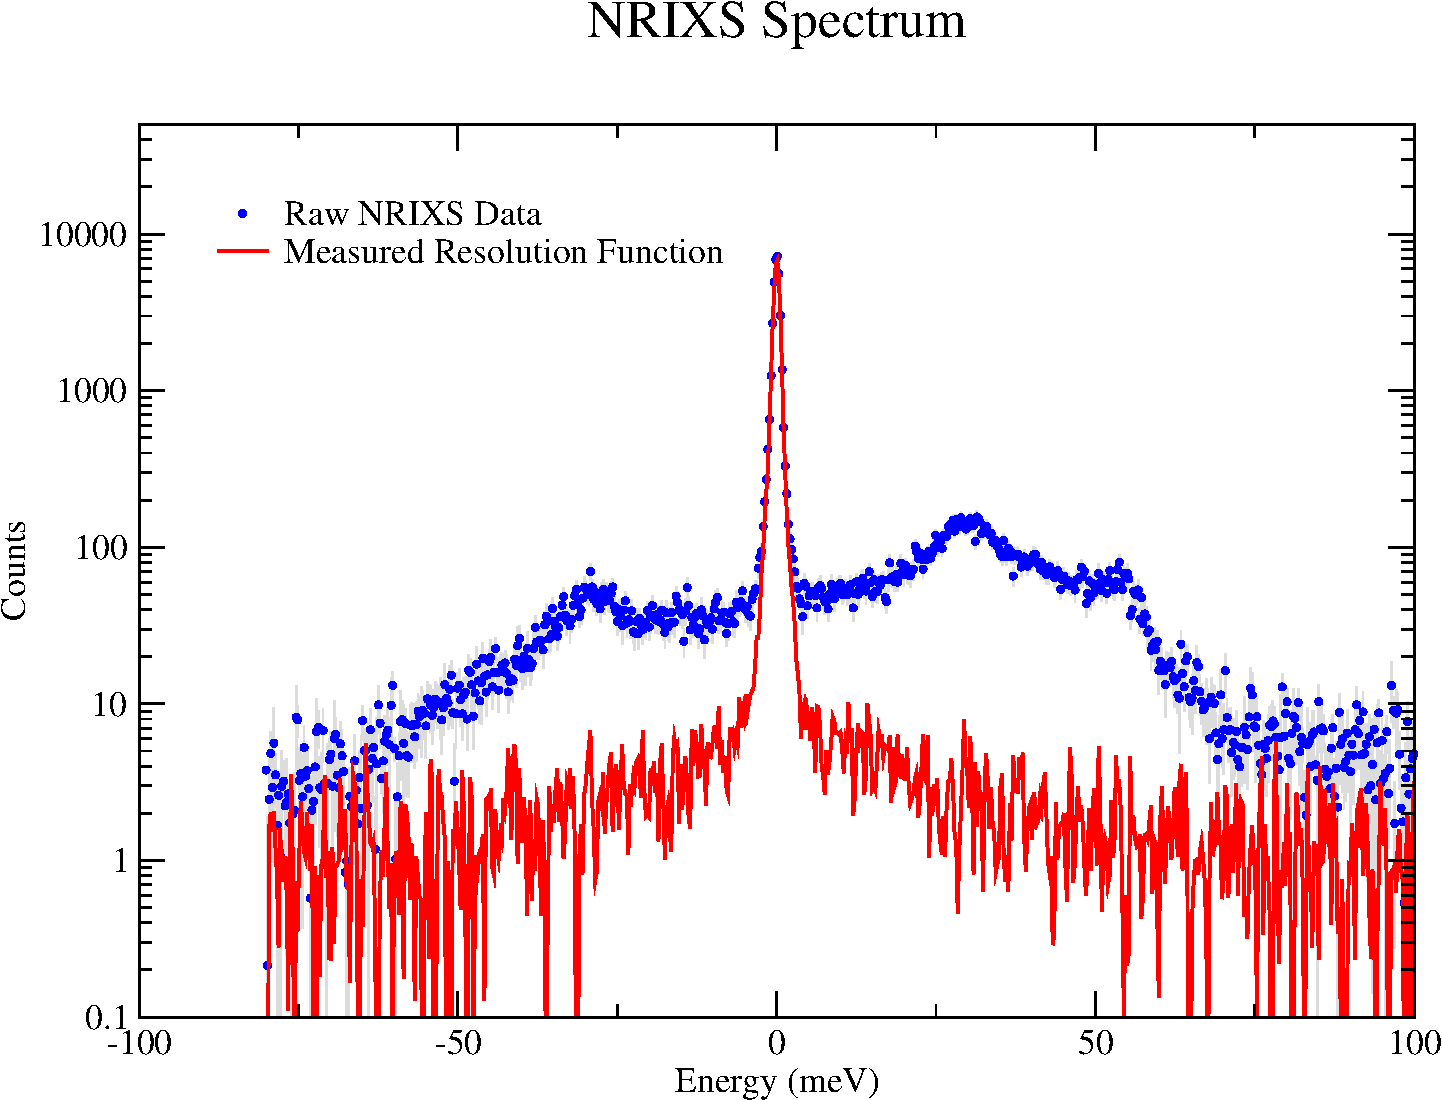
\includegraphics[width=8.0cm]{2015Mar_DAC13_P6//PhoxFigures/NRIXS_FeNiSi_DAC13_P6.pdf}} \quad
\subfloat{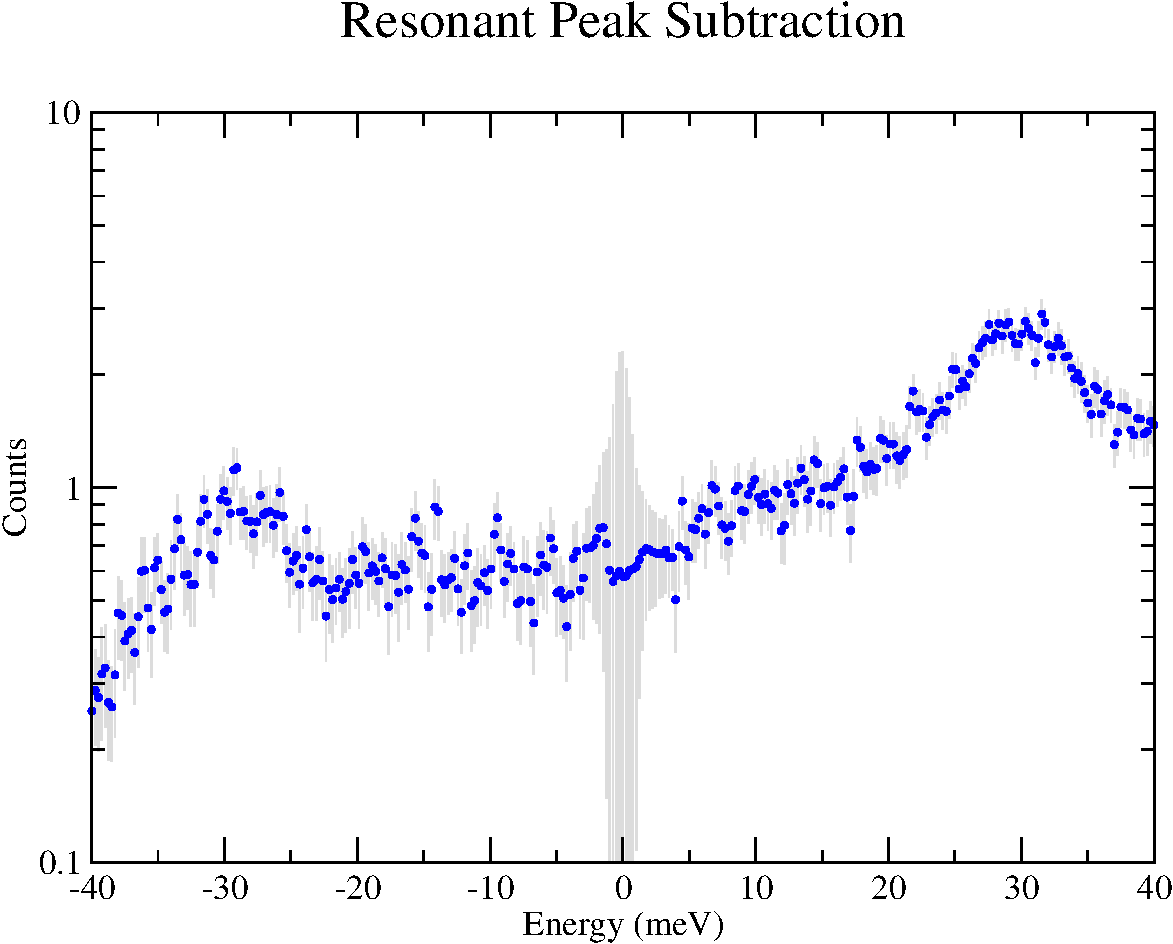
\includegraphics[width=7.5cm]{2015Mar_DAC13_P6//PhoxFigures/PeakSub_FeNiSi_DAC13_P6.pdf}} \\
\subfloat{\includegraphics[width=7.5cm]{2015Mar_DAC13_P6//PhoxFigures/PDOS_FeNiSi_DAC13_P6.pdf}} \quad
\subfloat{\includegraphics[width=7.5cm]{2015Mar_DAC13_P6//PhoxFigures/IntPDOS_FeNiSi_DAC13_P6.pdf}} \\
\subfloat{\includegraphics[width=8.0cm]{2015Mar_DAC13_P6//PhoxFigures/IntPDOSZoom_FeNiSi_DAC13_P6.pdf}} \quad
\subfloat{\includegraphics[width=7.5cm]{2015Mar_DAC13_P6//PhoxFigures/ResPeak_FeNiSi_DAC13_P6.pdf}}
\caption{PHOENIX phox data for Fe$_{0.80}$Ni$_{0.10}$Ni$_{0.10}$ data point FeNiSi\_DAC13\_P6.}
\label{fig:cont}
\end{figure}



\end{document}  				
